\chapter{Methodology Part 2: Advancing Several Layers}

In the previous chapter, we talked about how the very first layer of the mesh is generated. Starting from the discussion of extruding one boundary vertex onto the sub-surface, we discussed how all the vertices on the boundary curve of the sub-surface are extruded and subsequently, how the advancing front is recovered so that we can move on to the next layer. We also talked about how extrusion length scaling at concave corners helps us avoid immediate front collapse and improves overall mesh quality. In this chapter, we are going to discuss some of the important subroutines which help complete the anisotropic surface mesh.

We will start by discussing the subroutine used to control the aspect ratio as we advance several layers in the mesh. Combining triangular mesh elements to quad elements will be discussed next. Subsequently, mesh smoothing and collision handling will be discussed.

\section{Aspect Ratio Control and Sub-surface Interior Improvement}

\subsection{Vertex Decimation on the Front}
\label{aspectRatioControl}

As the advancing front moves into the surface interior, the layers grow in size. This is done to give a higher refinement at the boundary curves. As the size of the layer grows, the aspect ratio of the mesh elements generated decreases. Some of the vertices on the front may become so close to each other that the aspect ratio approaches unity. Growing the layers further with all the vertices on the front would lead to anisotropy in the orthogonal direction and/or front overlap. Hence, the decimation of some of the front vertices is necessary to proceed with the next few layers.

\begin{figure}[hbt!]
	\centering
	\begin{subfigure}{.5\textwidth}
		\centering
		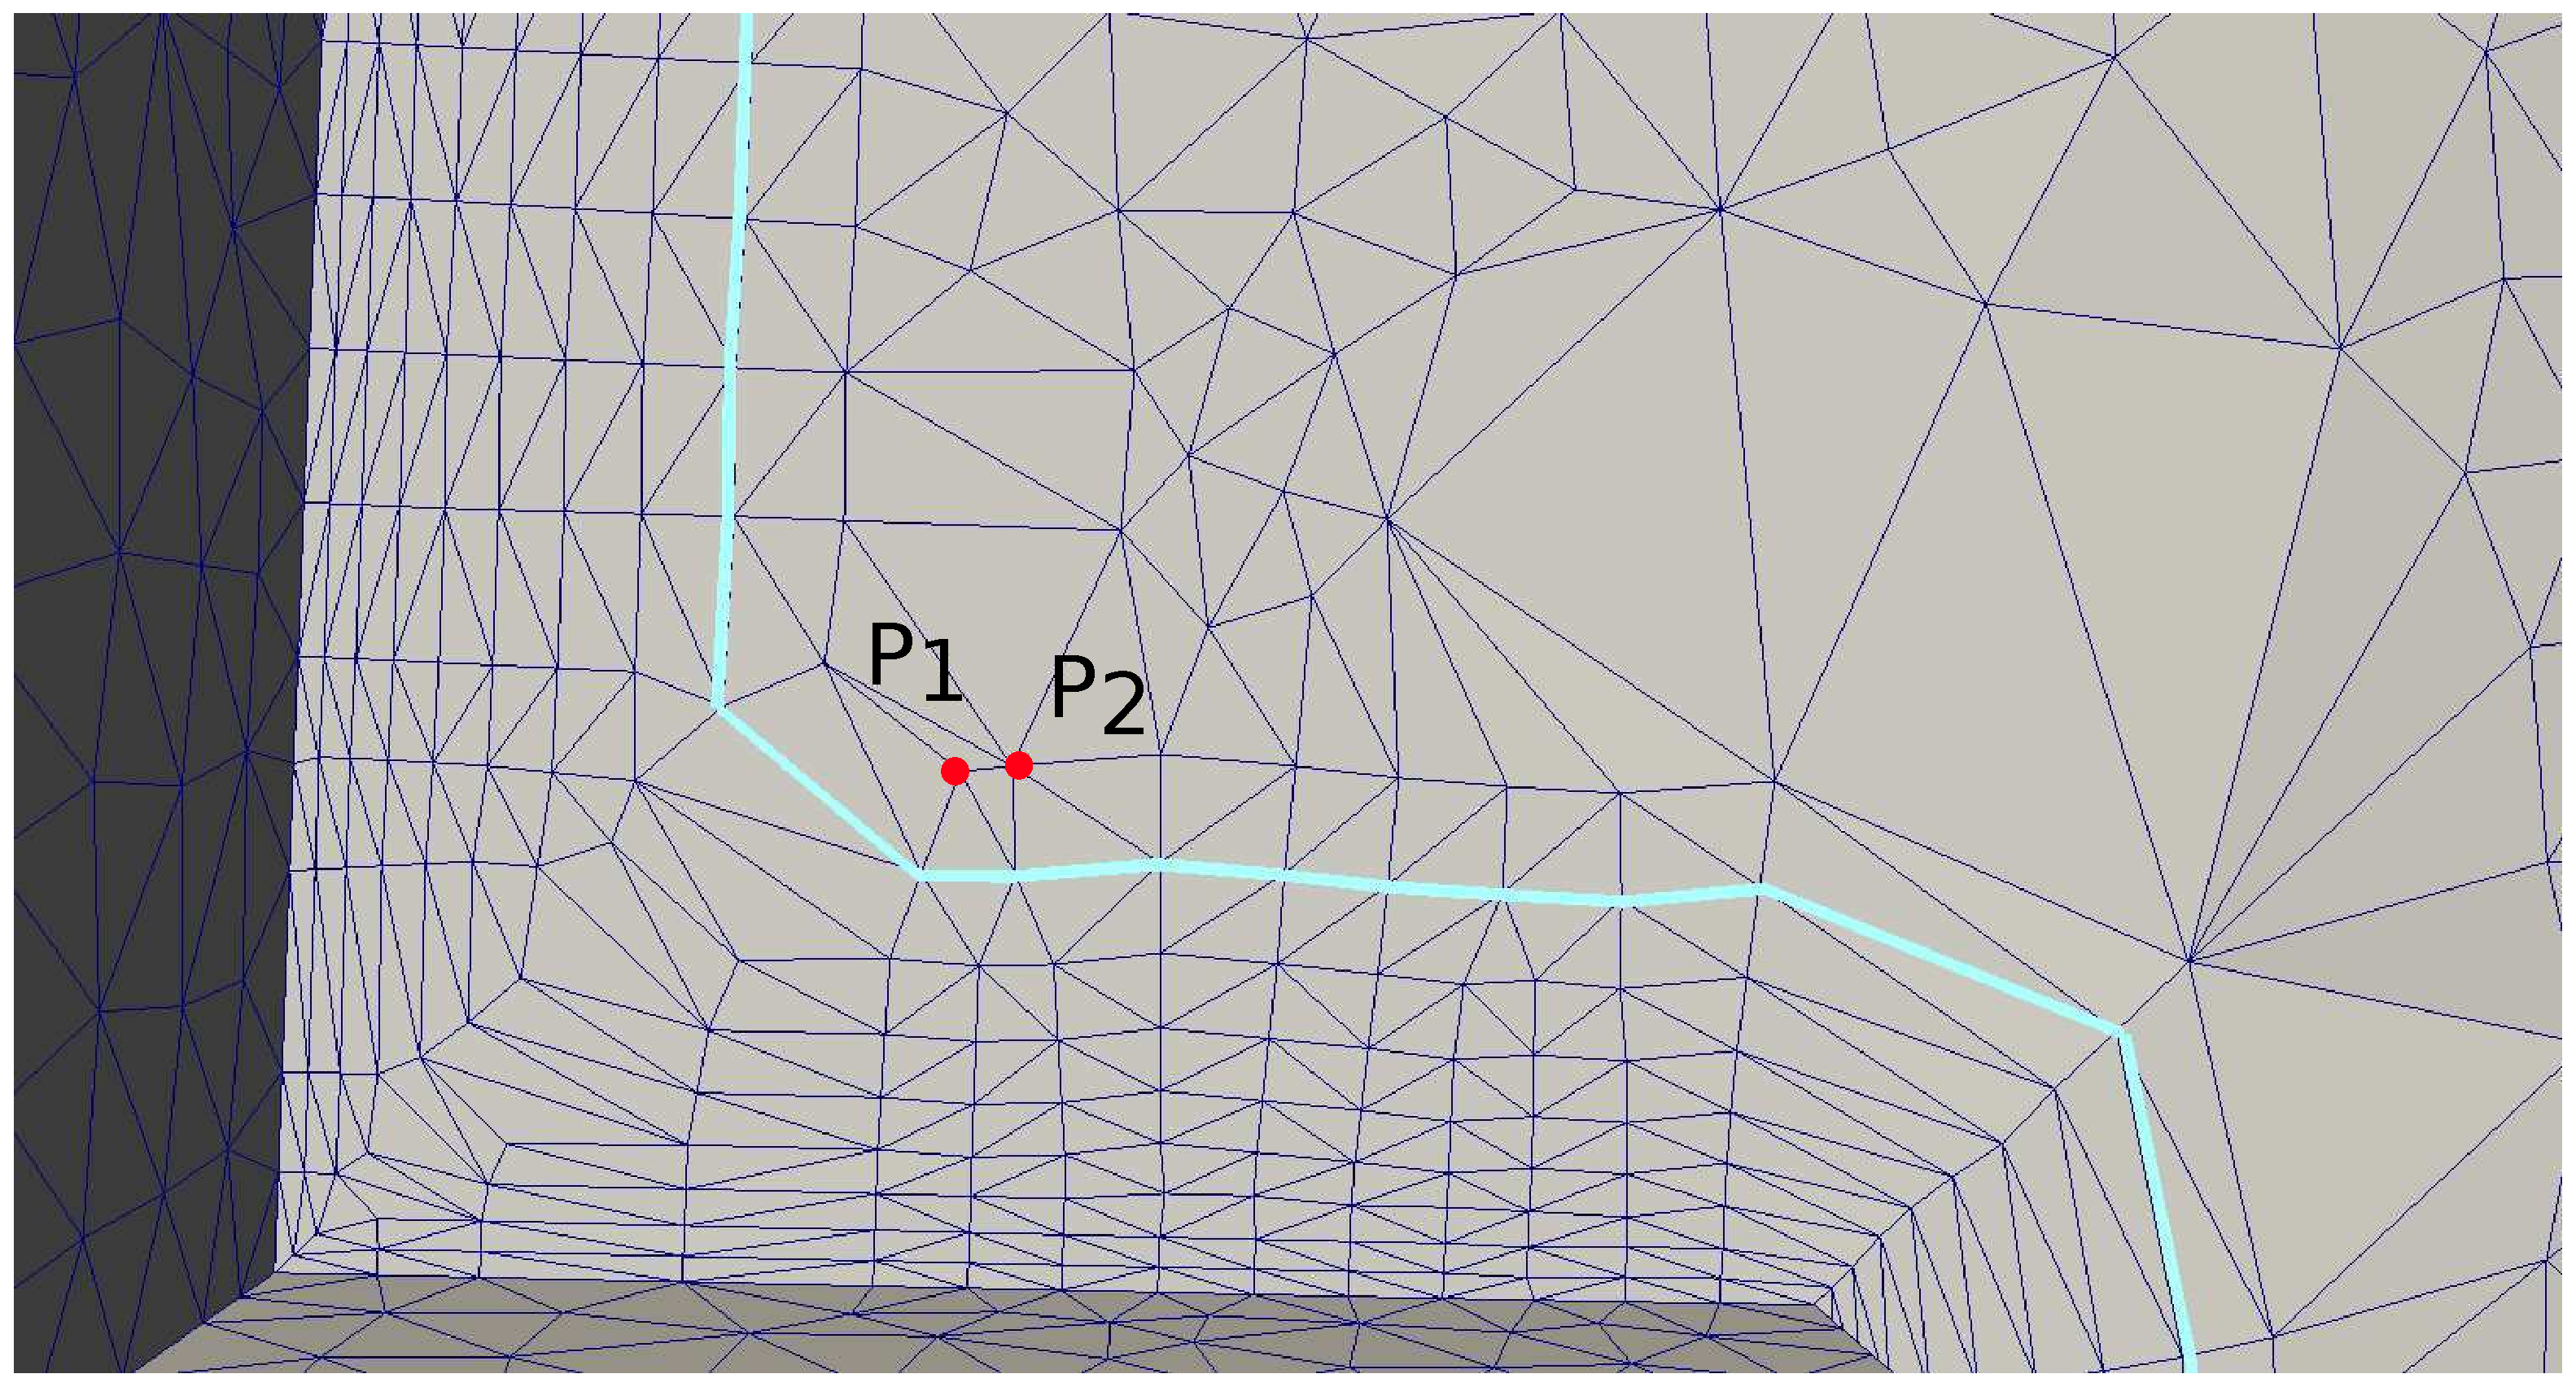
\includegraphics[width=.9\linewidth]{img/m2/edge-collapse/collapse1.eps}
		\caption{}
		\label{collapse1}
	\end{subfigure}%
	\begin{subfigure}{.5\textwidth}
		\centering
		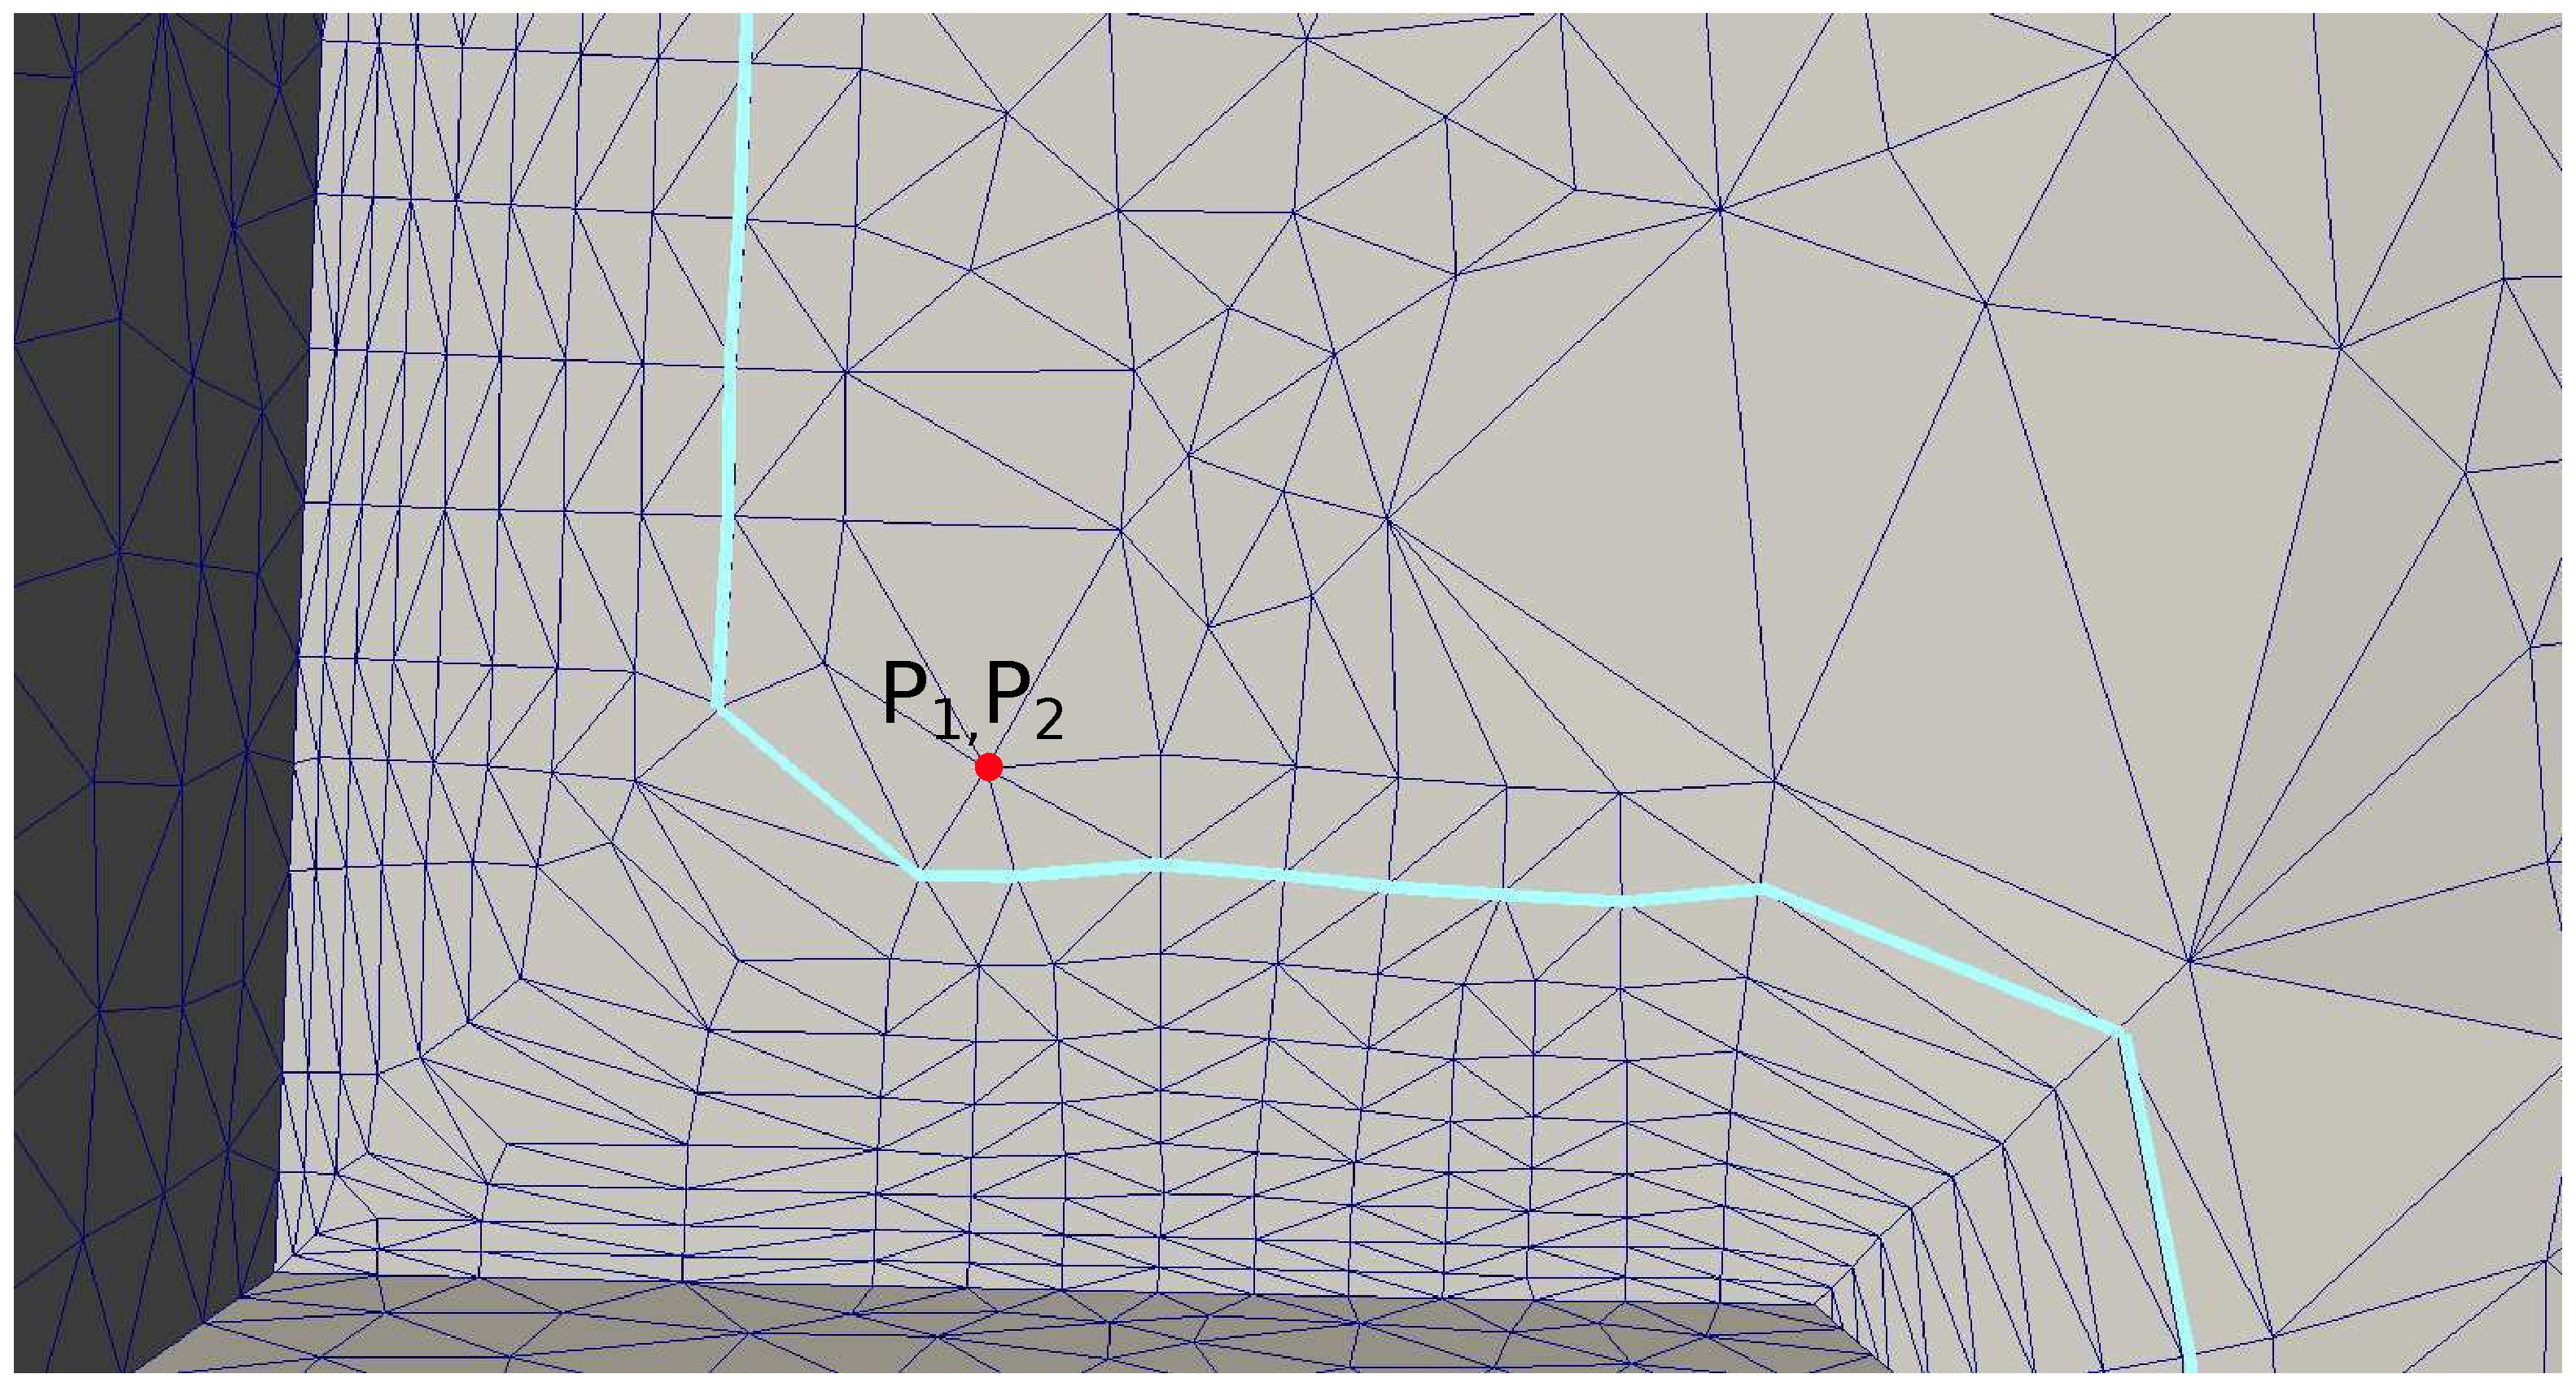
\includegraphics[width=.9\linewidth]{img/m2/edge-collapse/collapse2.eps}
		\caption{}
		\label{collapse2}
	\end{subfigure}
	\begin{subfigure}{.5\textwidth}
		\centering
		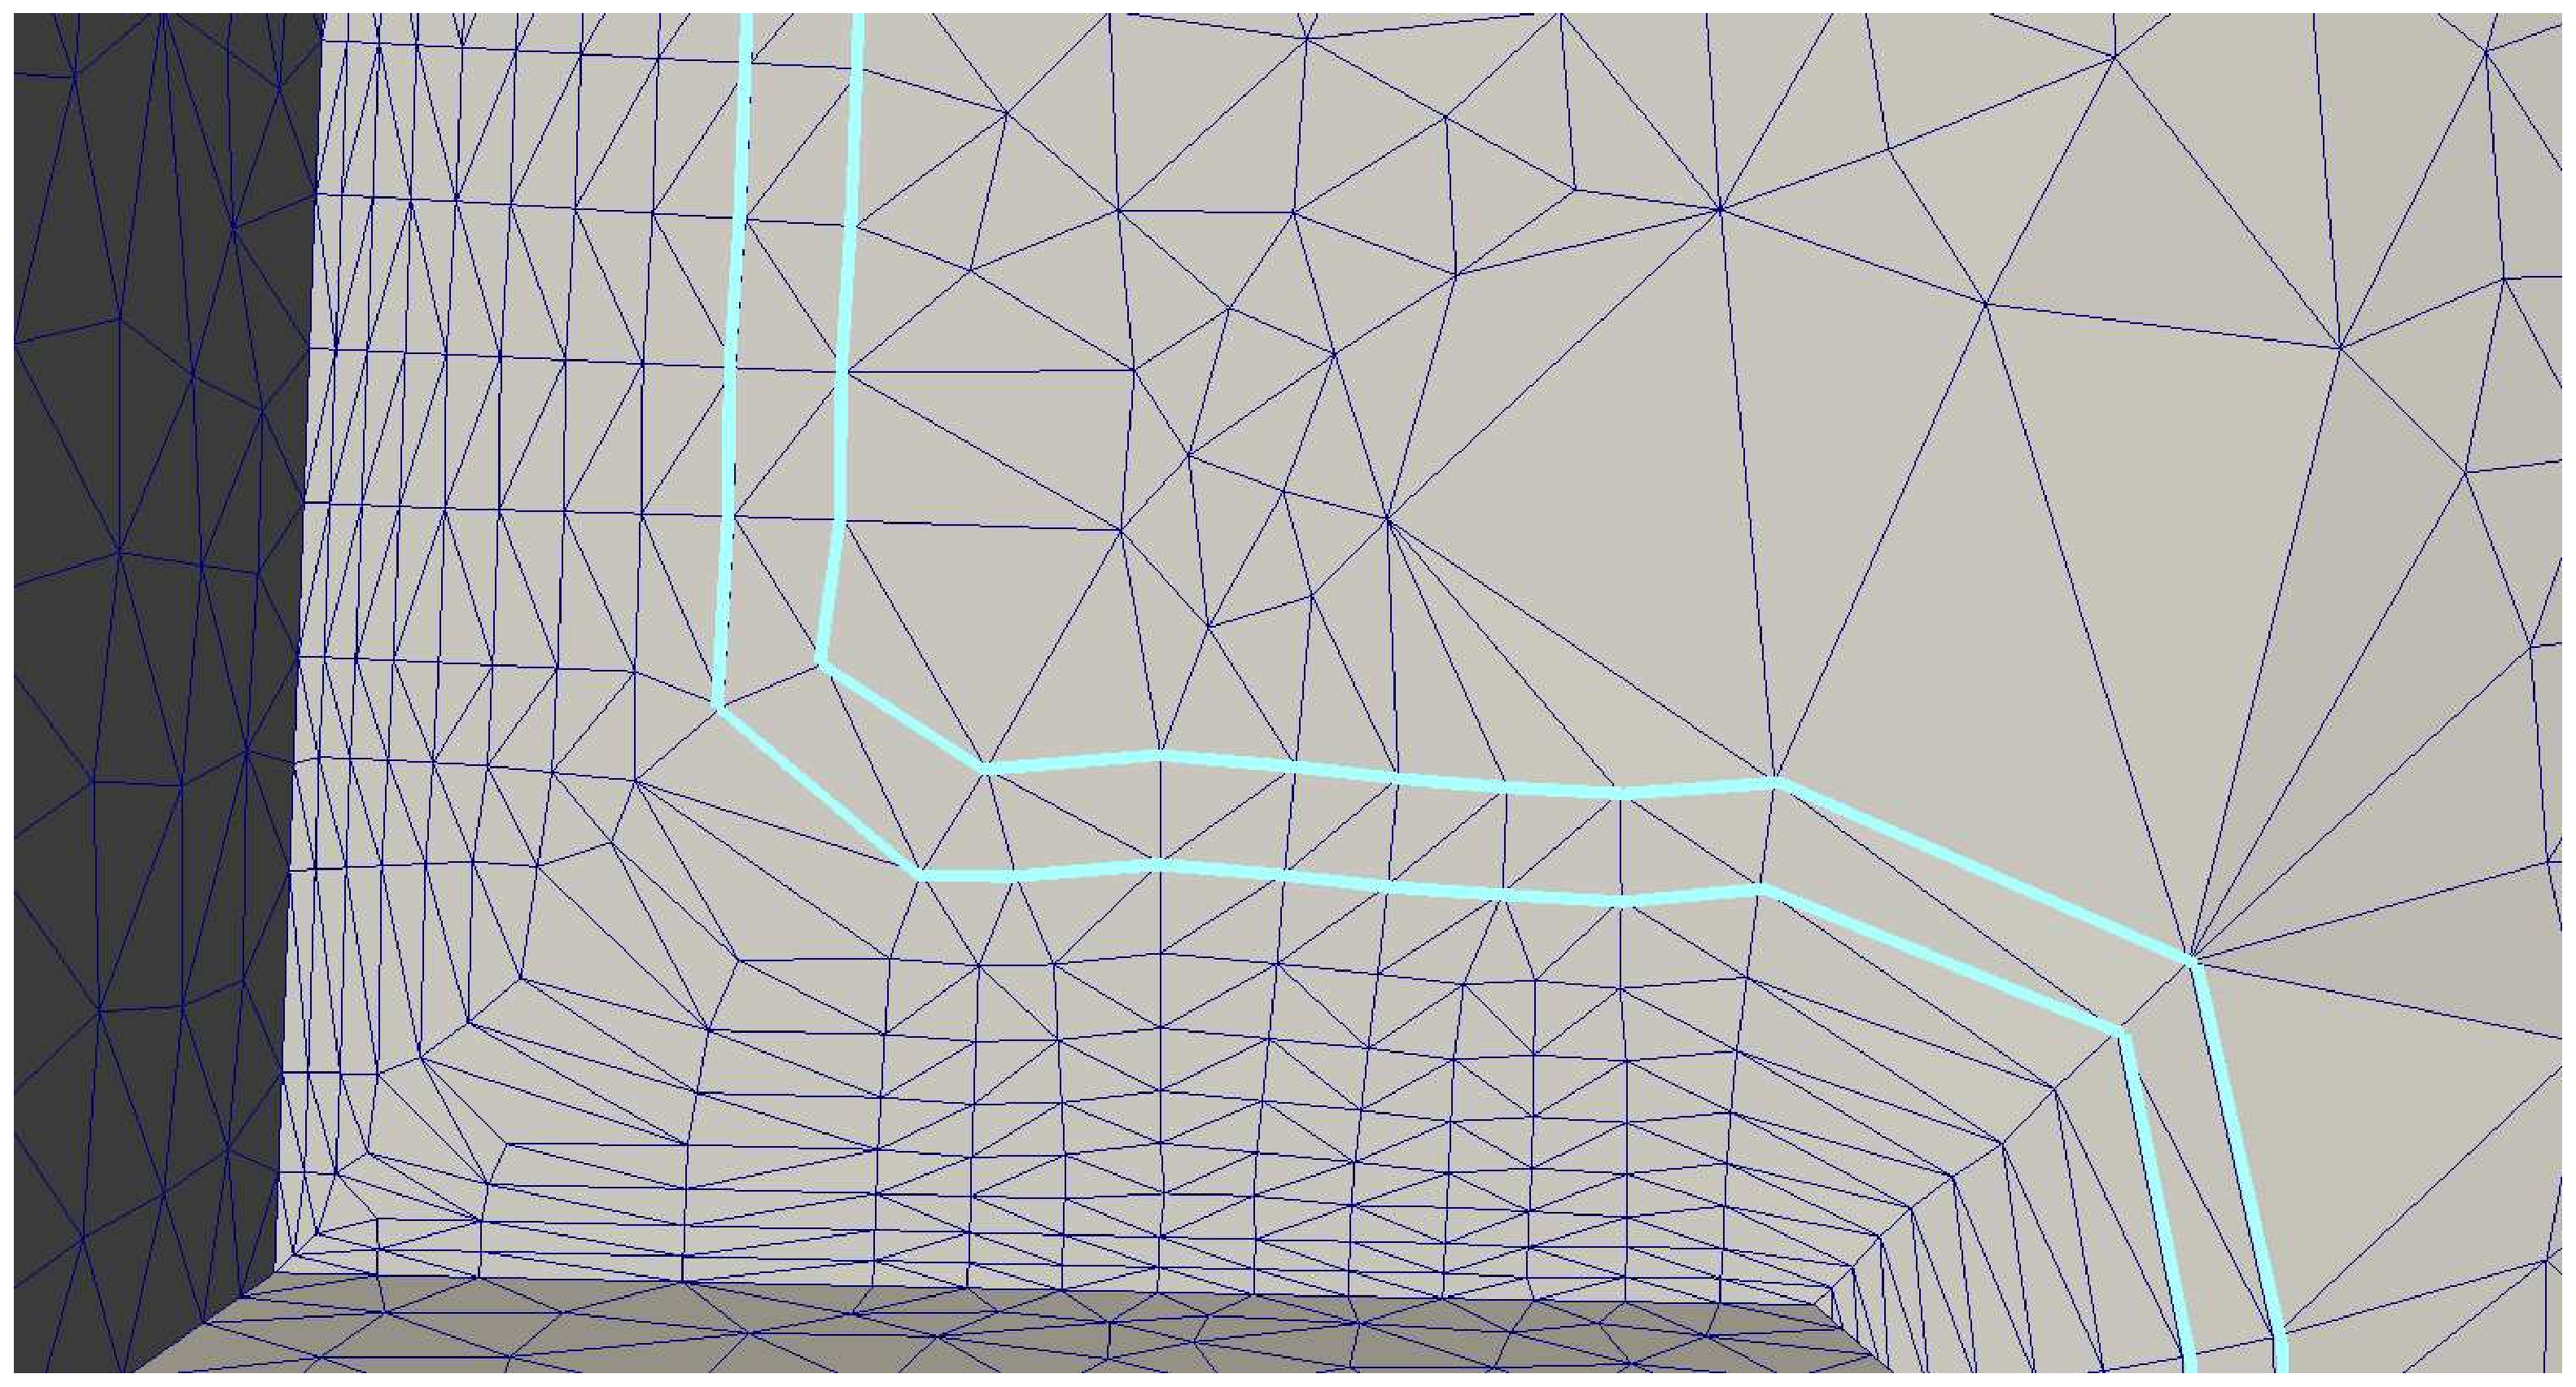
\includegraphics[width=.9\linewidth]{img/m2/edge-collapse/collapse3.eps}
		\caption{}
		\label{collapse3}
	\end{subfigure}
	\caption[Vertex decimation on advancing front to maintain aspect ratio.]{Edge collapse on an advancing front to avoid encroachment of points. In (a), two points in the kid layer $P_1$ and $P_2$ are too close to each other. Their parent layer is highlighted. If both the points advance to the next layer, then the next front would fail to recover. Hence, the edge between them is chosen to collapse. (b) shows the result of the edge collapse. The new location of both points is the average position of their initial location. (c) shows how the next front looks.}
	\label{edge-collapse}
\end{figure}

Once we have recovered the advancing front by iterative edge swaps to connect the kid points in the mesh, we check for vertices on the front that are too close to each other relative to the extrusion length. For instance, vertices that are near a concave corner could encroach each other if they are not decimated. Another example of a situation where vertex decimation on the advancing front becomes necessary is when the front has advanced to a substantial distance from the surface boundaries. In such a case, the extrusion length on the front has grown so much that the aspect ratio approaches unity. Decimating vertices from the front which are at a substantial distance from surface boundaries helps prevent the cell aspect ratio, ie front edge length over extrusion length, from dropping below one.

To check for vertices to decimate, we iterate through the vertices on the front and identify the ones which are too close to their neighbors. Vertex decimation is done through the conventional edge-collapse subroutine as described in \cite{hoppe1994mesh}. The threshold edge length between two points on the front is set to be $2 \tan(\pi/8)$ times the average extrusion length at those points. This value is set in order to minimize the normalized maximum deviation of angle from $90^\circ$ for quad elements. Hence, the threshold ensures that the anisotropic properties are retained for several layers while marching onto the surface. All short edges on the front are collapsed using the edge-collapse algorithm. An example of an edge-collapse on the front is shown in Figure \ref{edge-collapse}. Here, two points $P_1$ and $P_2$ are collapsed into a single point which forms a part of the next front on the surface. Mathematically,

\begin{equation}
l_{\mathit{collapse}} = 2 \; \tan \left( \frac{pi}{8} \right) \; x_n \; ;
\end{equation}

where $l_{\mathit{collapse}}$ is the minimum length of an edge on the advancing front which will not be considered for collapse and $x_n$ is the extrusion length at the $n^{th}$ layer.

%Validation checks are made before collapsing an edge. The deviation of the triangles formed as a result of edge collapse from the underlying surface is constrained to be less than $30^{\circ}$ to limit the deviation of the mesh from the ground truth surface $S$. 

Topological and geometrical checks are done before an edge can be collapsed in the mesh. These include a threshold for the ratio of the area of generated triangles and a limit on the dihedral angle between the adjacent triangles created by the collapse. The area threshold is set to be $10^8$. Also, edge-collapse is successful only if the triangles resulting from it are within a limit of $\theta < 30^{\circ}$ from the underlying surface (see Figure \ref{deviation-surface}). Lastly, there is a threshold for the maximum dihedral angle between any two adjacent triangles that result from the edge-collapse. This threshold is set to $40^{\circ}$. 

After we have recovered the front and decimated encroaching vertices in the surface interior as well as on the advancing front through edge collapse, we queue up the immediate interior edges of the surface and swap them for maximizing mesh quality. This step is included so that we have a good interior triangulation at each step of the advancing layer routine. It ensures that we do not have skinny triangles ahead of the front which might cause problems as we continue to march.

The edge collapse subroutine on the advancing front helps in controlling the aspect ratio at the front and limit its minimum value to 1. Whenever the aspect ratio value approaches 1, some vertices are removed from the front to increase the aspect ratio and front marching continues. Additionally, at concave corners with low aspect ratios, the edge collapse subroutine helps in maintaining a valid front to continue marching towards the surface interior.

\subsection{Vertex Decimation in Sub-Surface Interior}

As discussed in the previous chapter, we follow a closed advancing front methodology to generate the anisotropic surface mesh. The input triangulation $T$, which is the encoding of the surface $S$, is taken to be the initial mesh. Such a technique helps us in maintaining a complete and valid surface mesh at each step in the mesh generation process. However, this means that we need to do some additional work in deleting the vertices on the sub-surface imported initially which are no longer required to be a part of the anisotropic surface mesh. Fortunately, we have all the connectivity information of the vertices on the front. This means that we do not have to scan the 3D space near the vertex to find the encroaching points. Checking the vertices in the surface interior which share an edge with a front vertex is sufficient.

\begin{figure}[hbt!]
	\centering
	\begin{subfigure}{.5\textwidth}
		\centering
		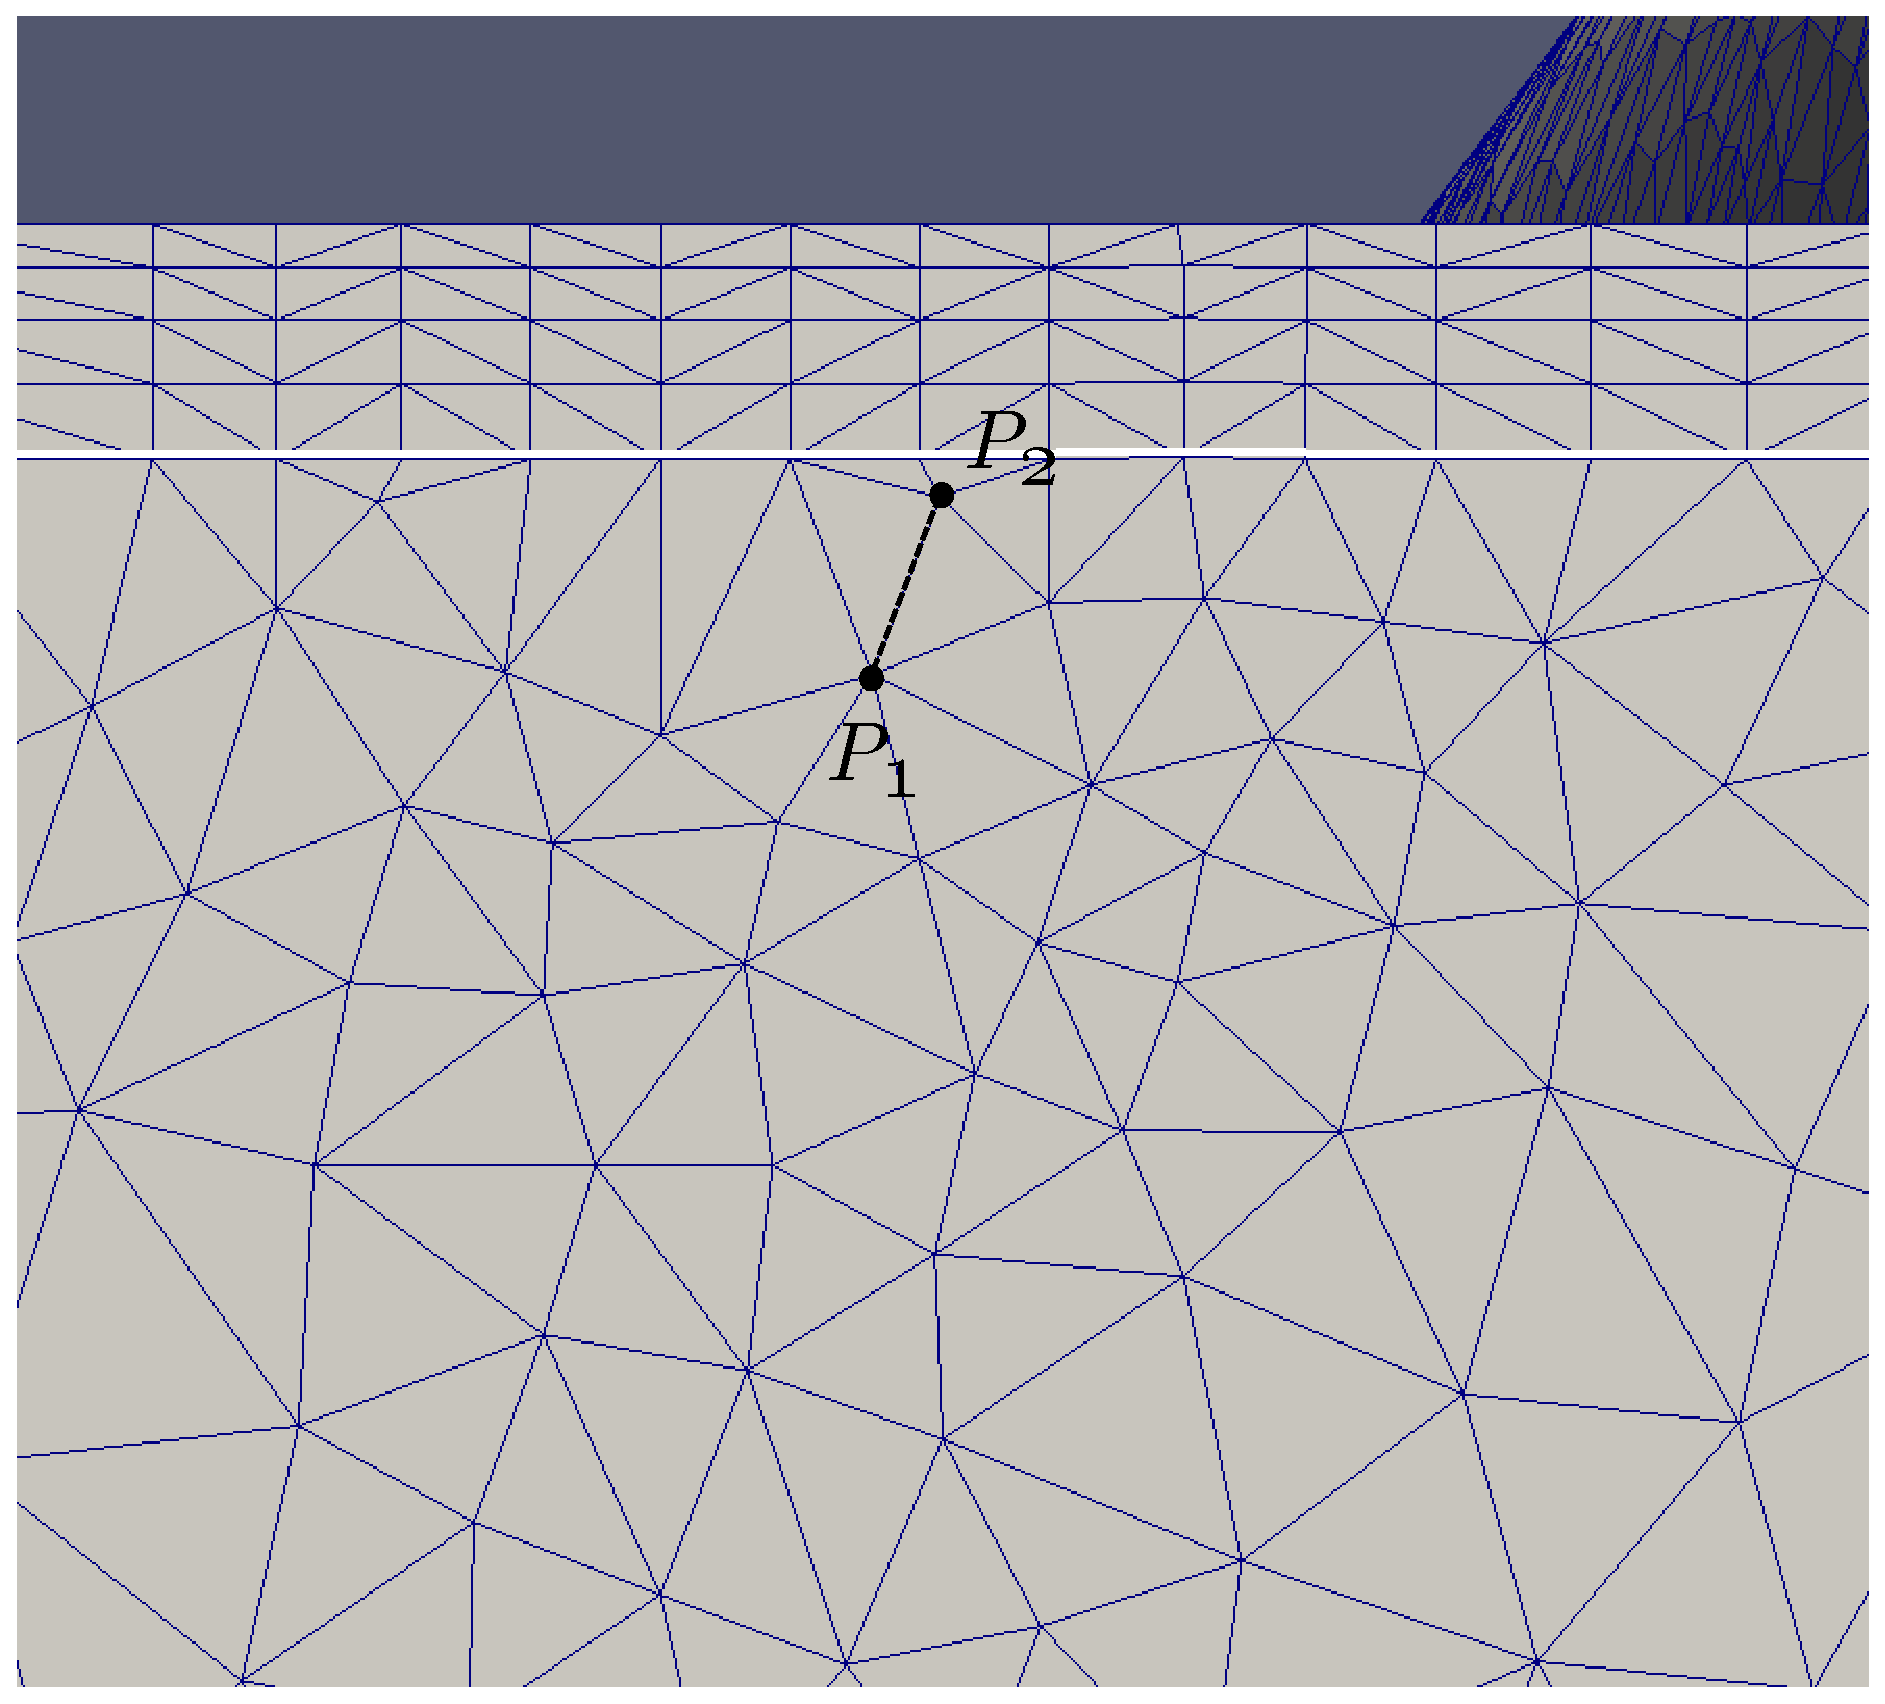
\includegraphics[width=.9\linewidth, trim={0 5cm 0  0}, clip]{img/m2/interior-vert-collapse/cc1.eps}
		\caption{}
		\label{cc1}
	\end{subfigure}%
	\begin{subfigure}{.5\textwidth}
		\centering
		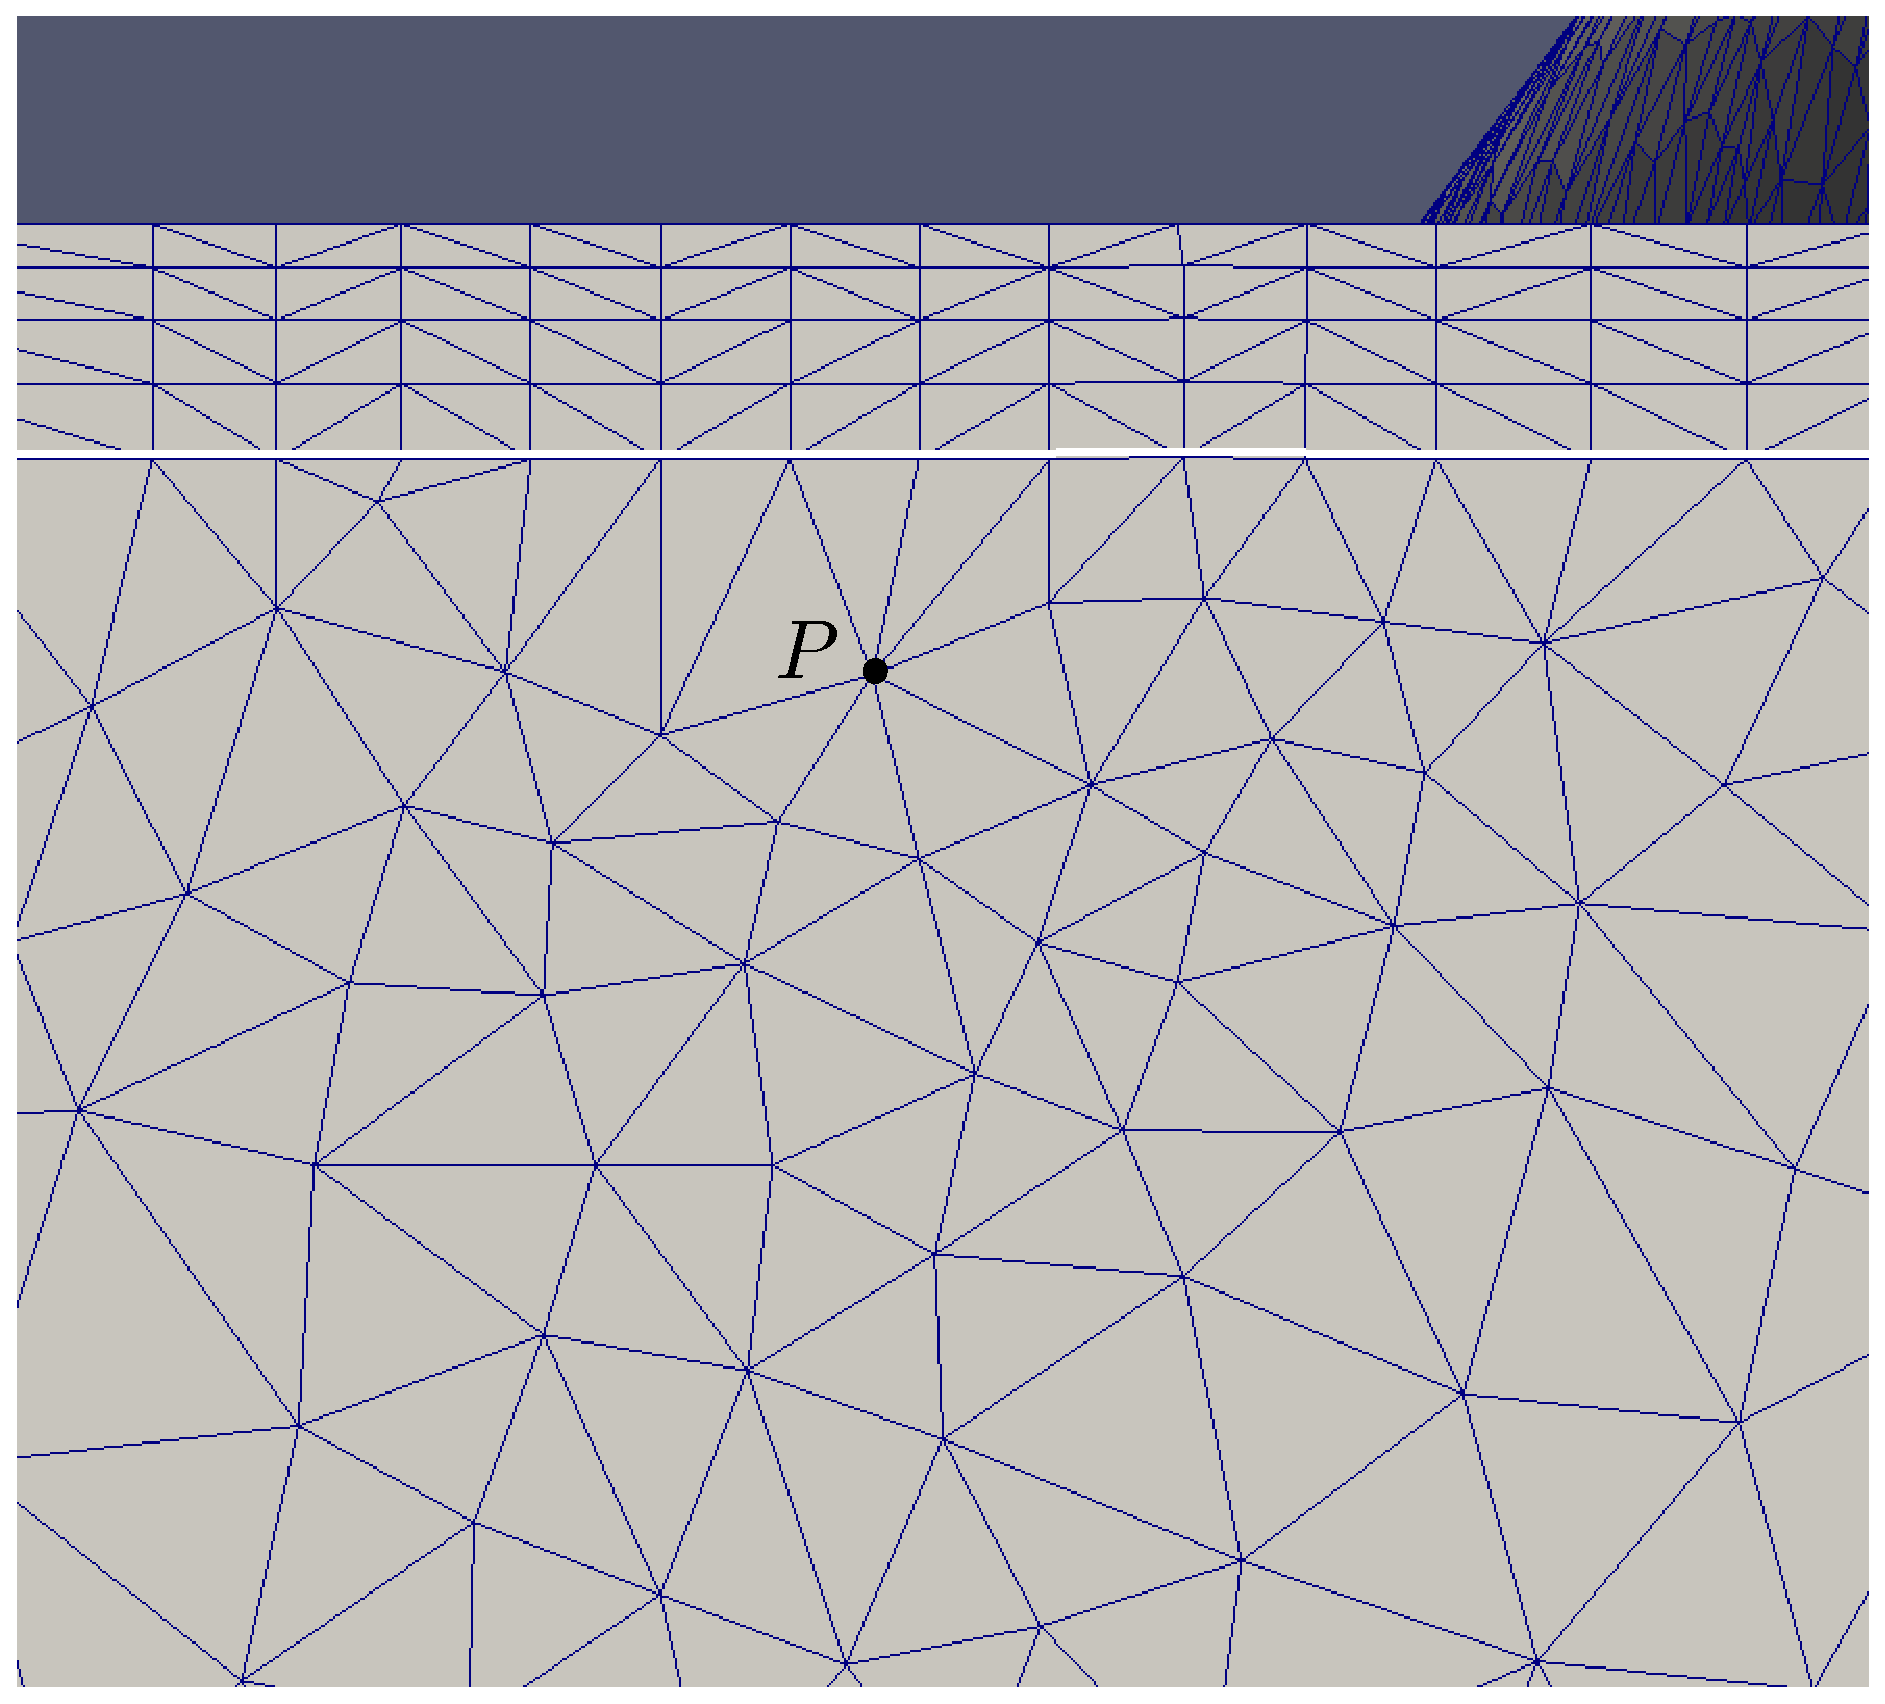
\includegraphics[width=.9\linewidth, trim={0 5cm 0  0}, clip]{img/m2/interior-vert-collapse/cc2.eps}
		\caption{}
		\label{cc2}
	\end{subfigure}
	\begin{subfigure}{.5\textwidth}
		\centering
		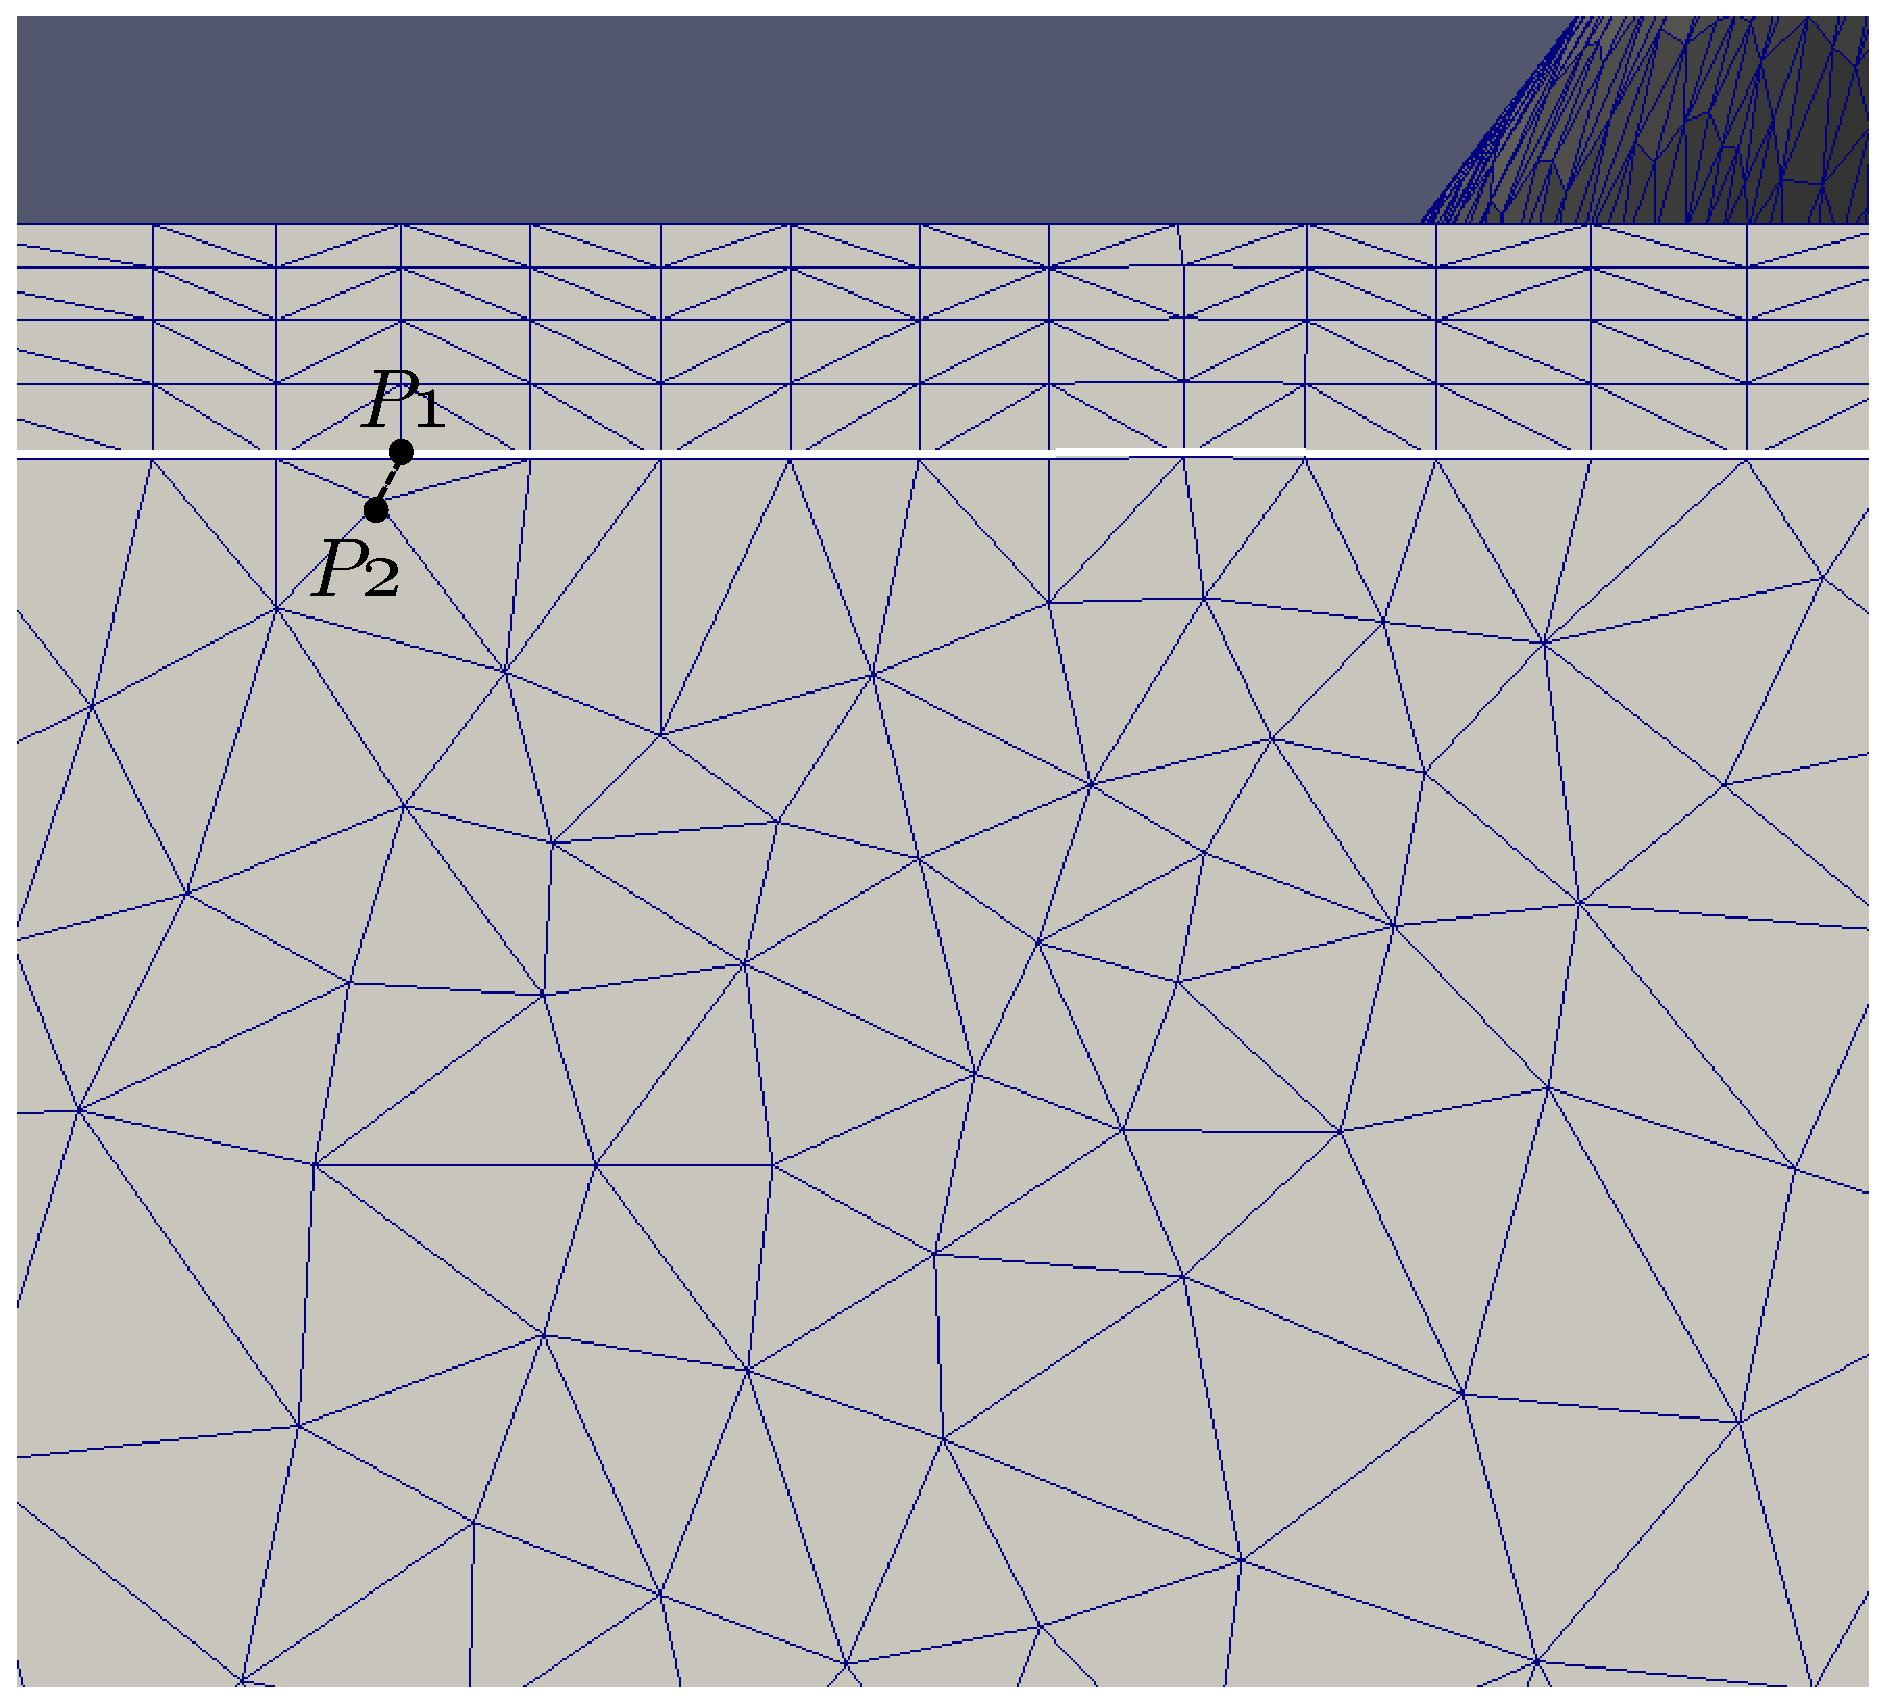
\includegraphics[width=.9\linewidth, trim={0 5cm 0  0}, clip]{img/m2/interior-vert-collapse/cc3.eps}
		\caption{}
		\label{cc3}
	\end{subfigure}%
	\begin{subfigure}{.5\textwidth}
		\centering
		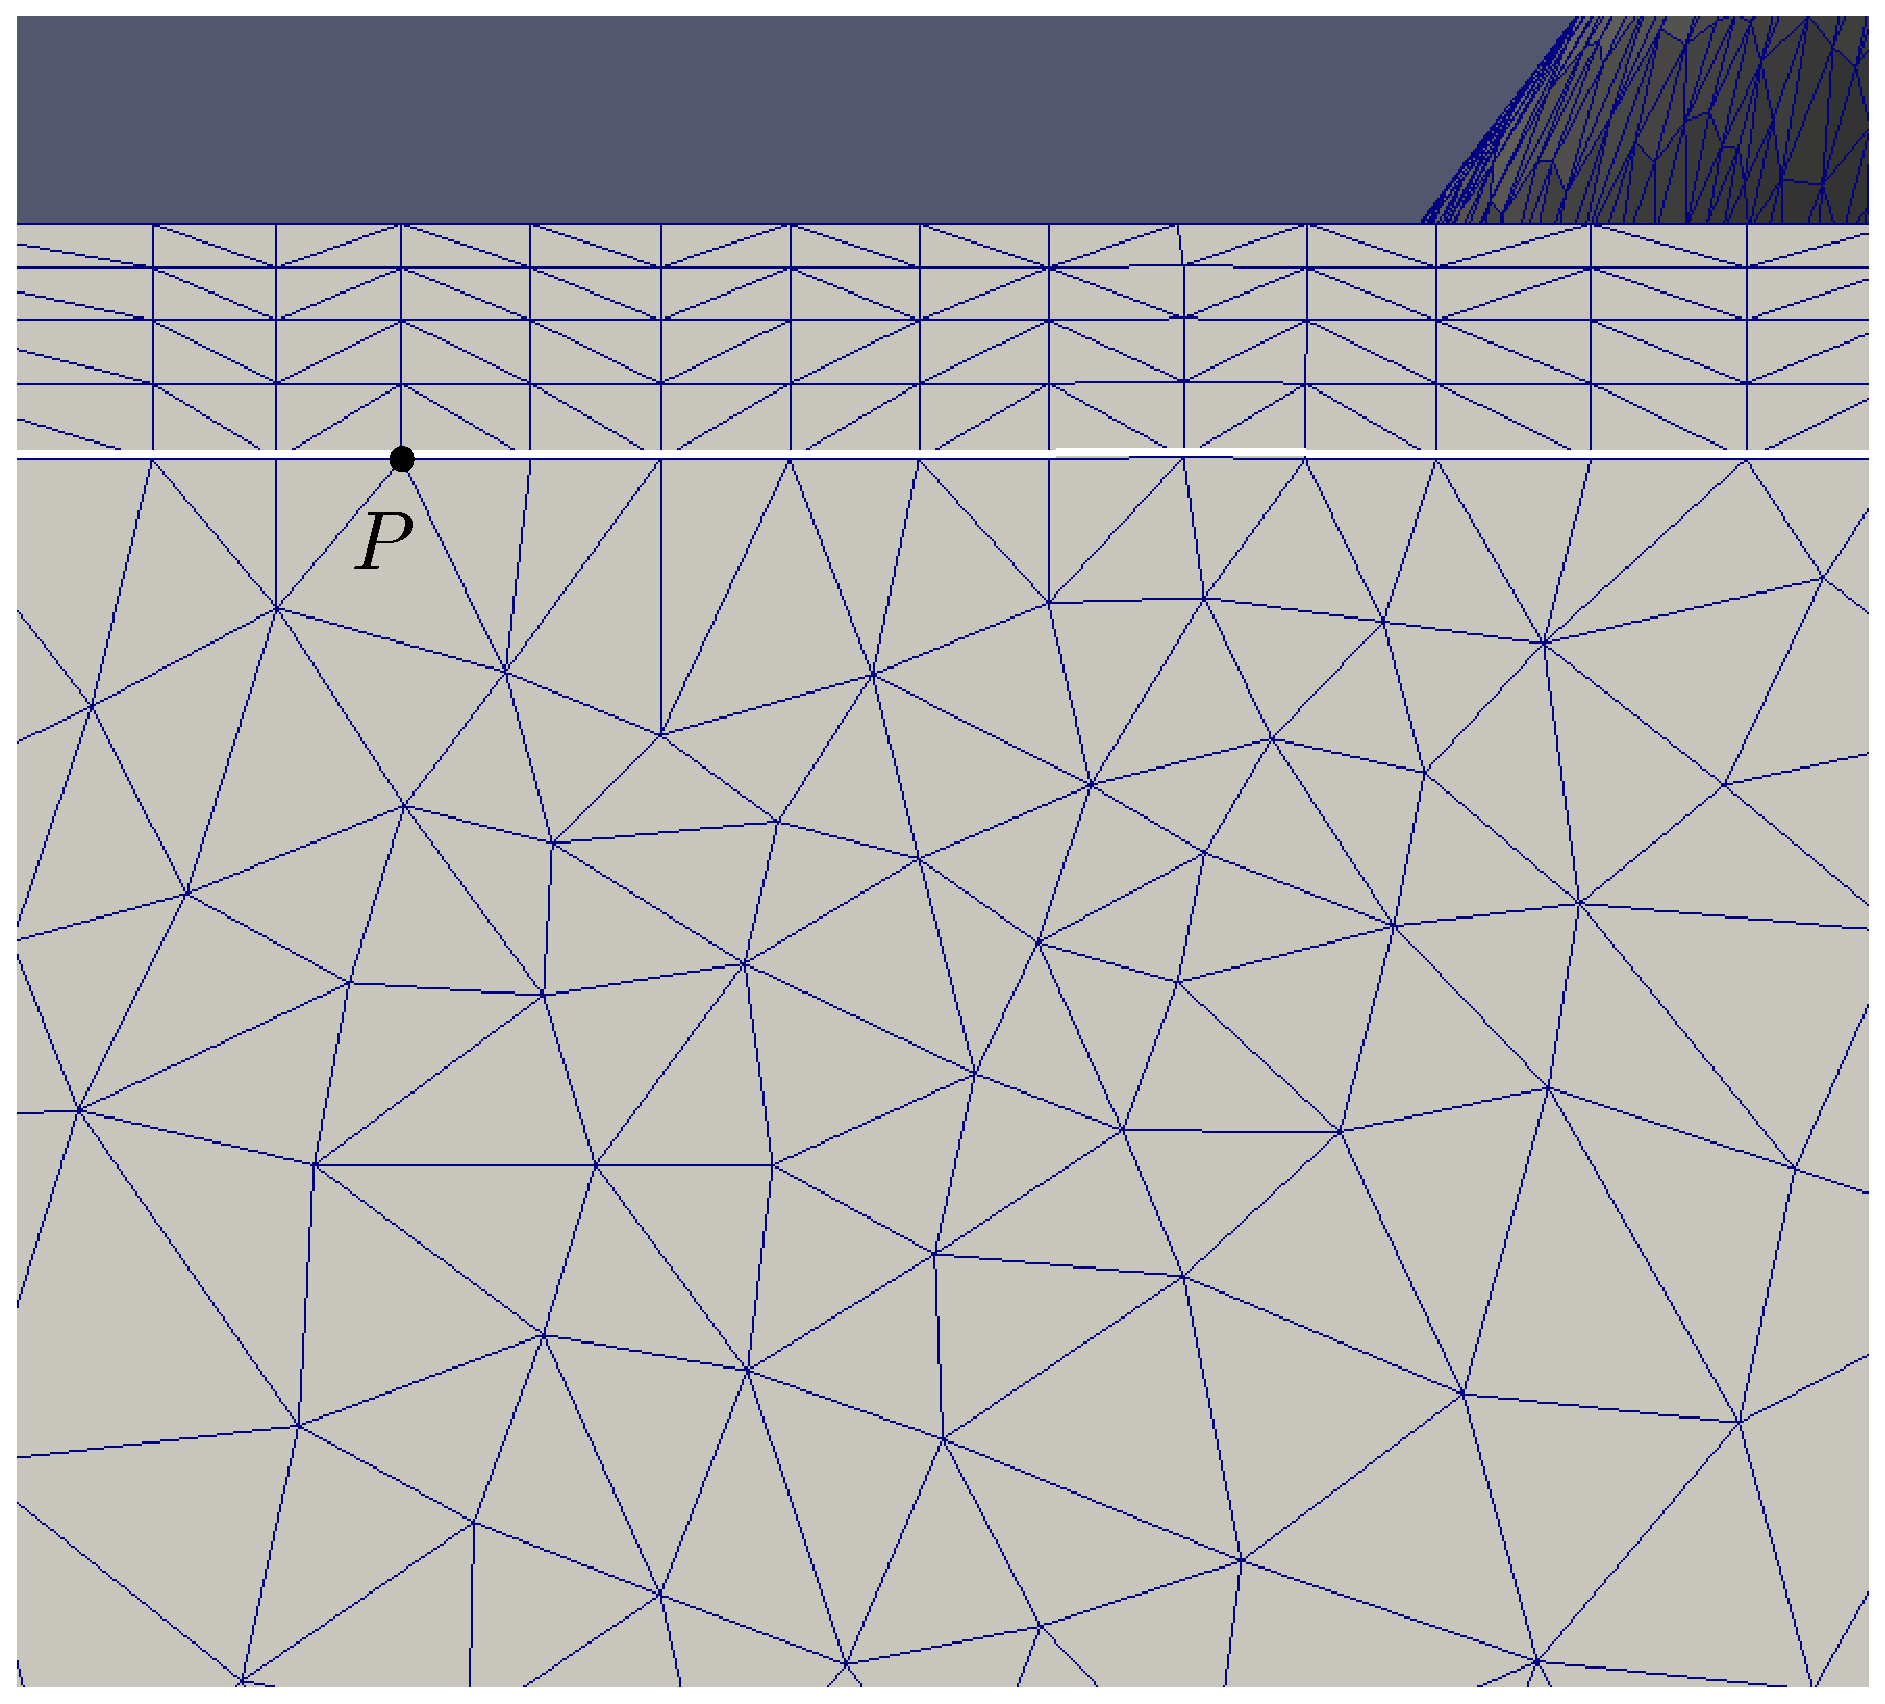
\includegraphics[width=.9\linewidth, trim={0 5cm 0  0}, clip]{img/m2/interior-vert-collapse/cc4.eps}
		\caption{}
		\label{cc4}
	\end{subfigure}
	\caption[Interior vertex decimation through edge collapse.]{Interior vertex decimation through edge collapse. The highlighted white line shows the advancing front. In (a), vertex $P_2$ is about to encroach the front. Hence, the best vertex for collapse is chosen among their neighbours. The best vertex for edge collapse here is $P_1$. Here, $P_2$ is collapsed on to $P_1$. The connectivity after the edge collapse is shown in (b) where vertex $P$ represents the collapsed vertex. Similarly, in (c), vertex $P_2$ is about to encroach the advancing front and is collapsed onto vertex $P_1$ which is on the advancing front itself. The new connectivity is shown in (d) where all the possibly encroaching vertices for the advancing layer are decimated.}
	\label{interior-vert-collapse}
\end{figure}

In other words, as the advancing front marches onto the surface, vertices in the interior of the surface immediately next to the front are decimated to make way for the advancing layers. Before extruding a point $P$ on the advancing front, we check if any point in the surface interior with which it shares an edge meets the following condition. If it does, we decimate the interior vertex.

\begin{equation}
d < max \left( \frac{l_{1}}{\sqrt{2}}, \, \frac{l_{2}}{\sqrt{2}}, \; c \:\mathit{x_n}\right)
\label{collapse-eq}
\end{equation}

Here $d$ is the distance between the point on the advancing front and the interior point, $l_1$ and $l_2$ are the lengths of adjacent front edges of the point on the front, c is a constant whose value is set as $2$ and $x_n$ is the extrusion length at the vertex on the $n^{th}$ front. This condition ensures the decimation of vertices in the surface interior which are close to the advancing front and avoids any encroachment of surface interior vertices on the advancing layers. 

Validation checks for front edge collapse mentioned in the last subsection are also run during interior edge collapse. The quality criterion used for interior edge collapse is the maximization of the minimum angle in the triangles thus produced. The best edge for the collapse is chosen when decimating the interior vertices using this quality criterion. This is in contrast to the vertex decimation on the advancing front where the candidate edge for the collapse is already identified. An illustrative example for surface interior vertex decimation can be seen in Figure \ref{interior-vert-collapse}. All the interior vertices on the surface which come in the way of the advancing layers are removed as the layers move closer to the vertex. In some situations, the vertex which needs to be removed might not satisfy the quality criterion for the present marching layer. In such cases, the vertex is left as it and is removed after marching the next layer, or the one after that. No interior vertices were noticed to be interfering with the advancing layers as the vertices for decimation were checked at each layer.

\section{Combining Triangular Elements to Quadrilateral Elements}

In section \ref{sec-simplicial}, we the pros and cons of simplicial and non-simplicial mesh elements. Then, in section \ref{consolidate-motivation}, we talked about the motivation to produce a hybrid surface mesh which consists of both simplicial and non-simplicial mesh elements. Briefly, a hybrid anisotropic surface mesh which consists primarily of quadrilateral elements with a small number of triangular elements gives us the flexibility to mesh topologically complex surface geometries while keeping the average vertex connectivity of the mesh to a low value.

Almost all vertices in our closed advancing front method have a parent-kid relationship. The successor of a vertex is called its kid while the predecessor is called the parent. There are a couple of exceptions to this. First, vertices on the boundary curve do not have a parent as they are the zeroth layer of the mesh. Second, wherever an edge collapse operation is done, two kids from two different parent vertices collapse into a single vertex. This leaves a kid vertex with two parents, or, in other words, two parents who share a common kid vertex.

\vspace{10pt}
\begin{figure}[hbt!]
	\centering
	\begin{subfigure}{\textwidth}
		\centering
		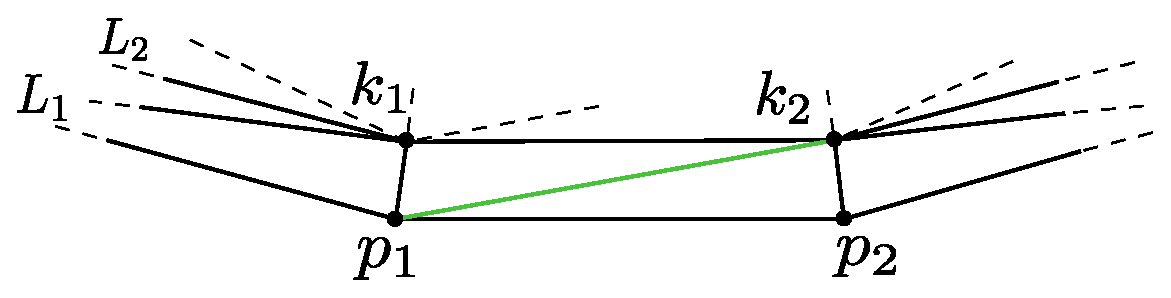
\includegraphics[width=.7\linewidth]{img/m2/combineTriToQuad.eps}
		\caption{}
		\label{triToQuad1}
	\end{subfigure}
	\begin{subfigure}{\textwidth}
		\centering
		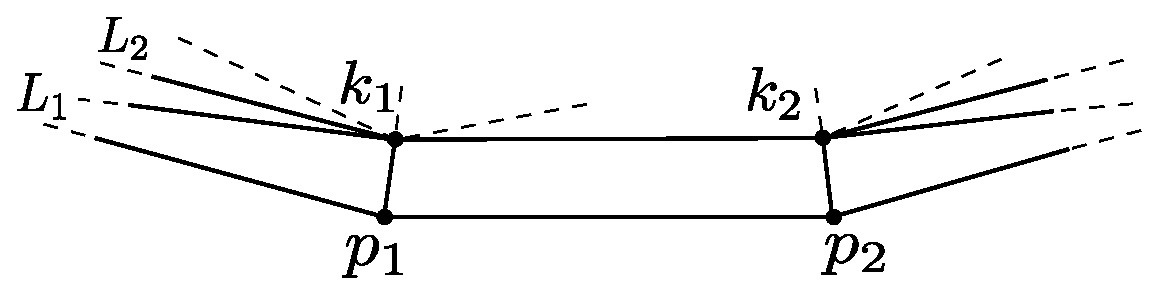
\includegraphics[width=.7\linewidth]{img/m2/combineTriToQuad2.eps}
		\caption{}
		\label{triToQuad2}
	\end{subfigure}
	\caption[Combining tris to quads]{Two triangles $\mathit{p_1k_1k_2}$ and $p_1p_2k_2$ are converted to a single quad $\mathit{p_1p_2k_2k_1}$.}
	\label{triToQuad}
\end{figure}

Apart from the two exceptions just mentioned, all the vertices have a parent and a kid. This gives some structure to our mesh. As the layers grow in the normal direction to the boundary curve, this helps us in generating rectangular quadrilateral elements easily. Edges are removed from the finished layers in order to generate superior-quality quadrilateral cells. As the layers advance from the boundary curves towards the tangential direction onto the surface, the quadrilateral elements generated retain the boundary topology several layers into the interior of the surface. The quality of a quadrilateral element is calculated as the inverse of the maximum deviation of its interior angles from 90 degrees. This criterion is selected to prefer rectangular elements and retain the boundary representation on the surface mesh. Starting from the first layer generated on the surface, multiple iterations of this subroutine are run for the same layer to ensure as few triangular elements are left per layer as possible.

Consider Figure \ref{triToQuad1}. $L_1$ and $L_2$ denote two successive layers on the advancing layer mesh. Points $p_1$ and $p_2$ are on the parent layer $L_1$ and their kids, $k_1$ and $k_2$, respectively, are on the kid layer $L_2$. All the edges in the neighborhood of $p_1$ and $p_2$ which are not on the advancing front and are not shared with their respective kids are queued. Then, these edges are sorted in order of the quality of the quadrilateral elements generated after their removal. Finally, all the edges in the queue are deleted. The edged marked in green in the figure is deleted in the process which results in the deletion of two triangular elements and generation of a new quadrilateral element. The local mesh after edge removal is shown in Figure \ref{triToQuad2}.

\vspace{10pt}
\begin{figure}[hbt!]
	\centering
	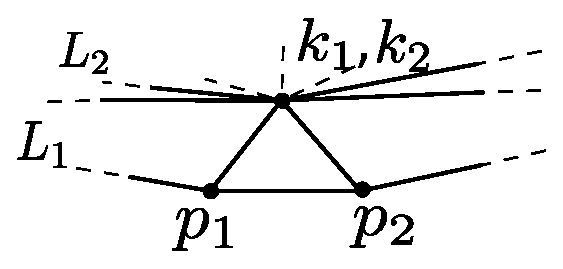
\includegraphics[width=0.5\linewidth]{img/m2/combineTriToQuad3.eps}
	\caption[Exception in combining tris to quads]{Sometimes, the subroutine responsible for maintaining aspect ratio combines two adjacent kid vertices to one. In such cases, we let the triangle remain on the advancing layer.}
	\label{triLeft}
\end{figure}

As discussed earlier, some exceptions exist in the advancing layer mesh where all the elements in a layer cannot be converted to a quadrilateral element. An illustration of such an exception is shown in Figure \ref{triLeft}. Here, two kids $k_1$ and $k_2$ had to collapse to a single vertex as the edge between them is collapsed in the aspect ratio control subroutine explained in section \ref{aspectRatioControl}. Hence, a triangle would be left in between layers $L_1$ and $L_2$. An example surface mesh that shows the result of combining triangular elements into quadrilateral elements can be seen in Figure \ref{fig-triQuad}. Most of the triangular mesh elements are converted to quadrilateral elements.

\begin{figure}
	\centering
	\begin{subfigure}{0.5\textwidth}
		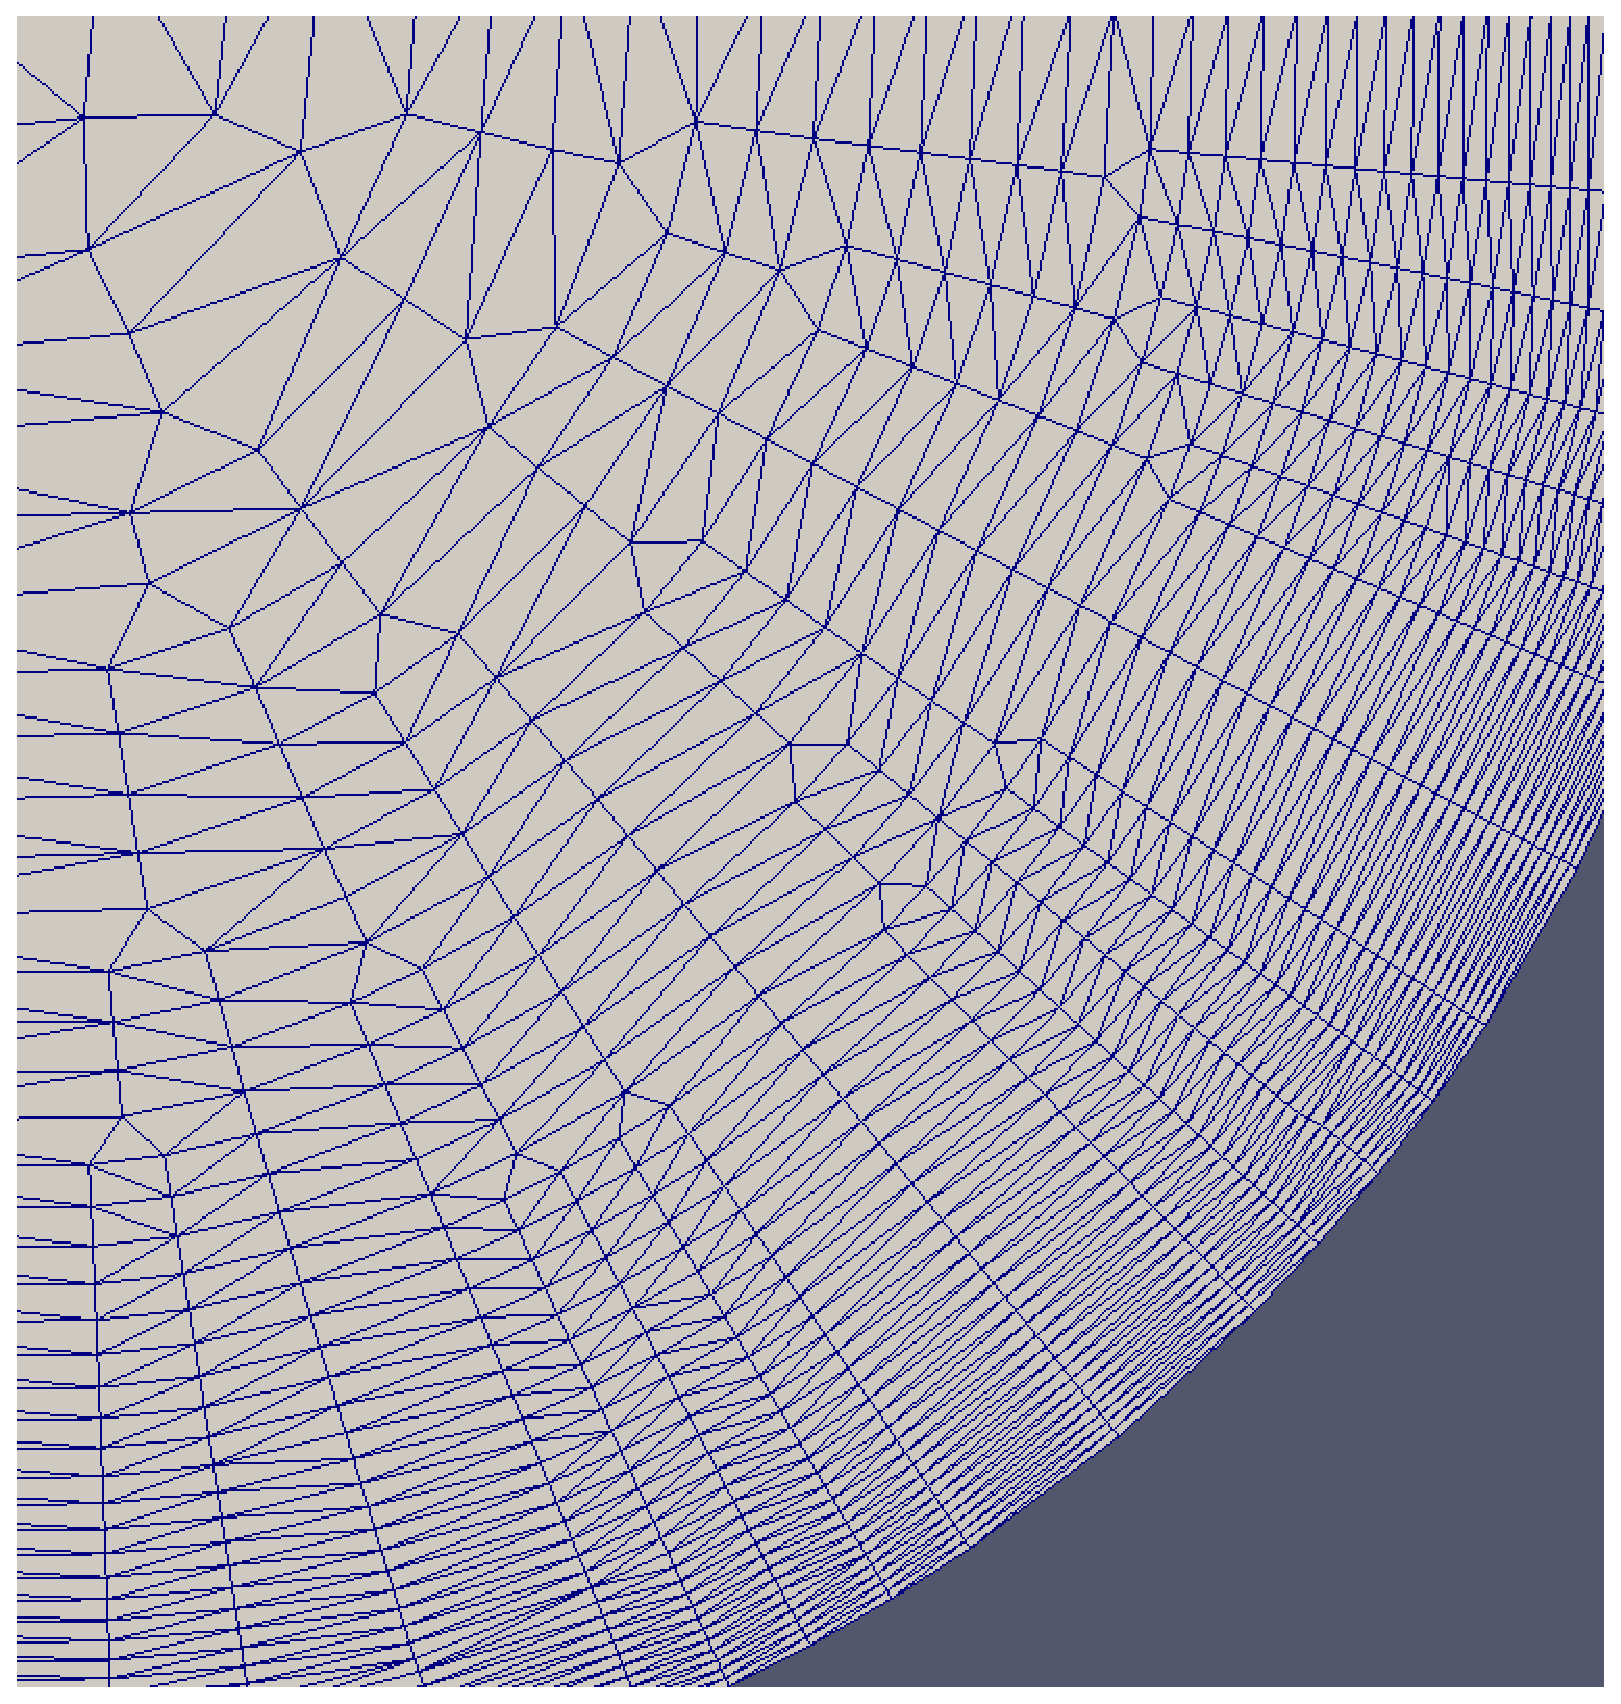
\includegraphics[width=0.9\linewidth]{img/m2/combine-tris-to-quads/combineTrisToQuads1.eps}
		\caption{}
		\label{fig-triQuad1}
	\end{subfigure}%
	\begin{subfigure}{0.5\textwidth}
		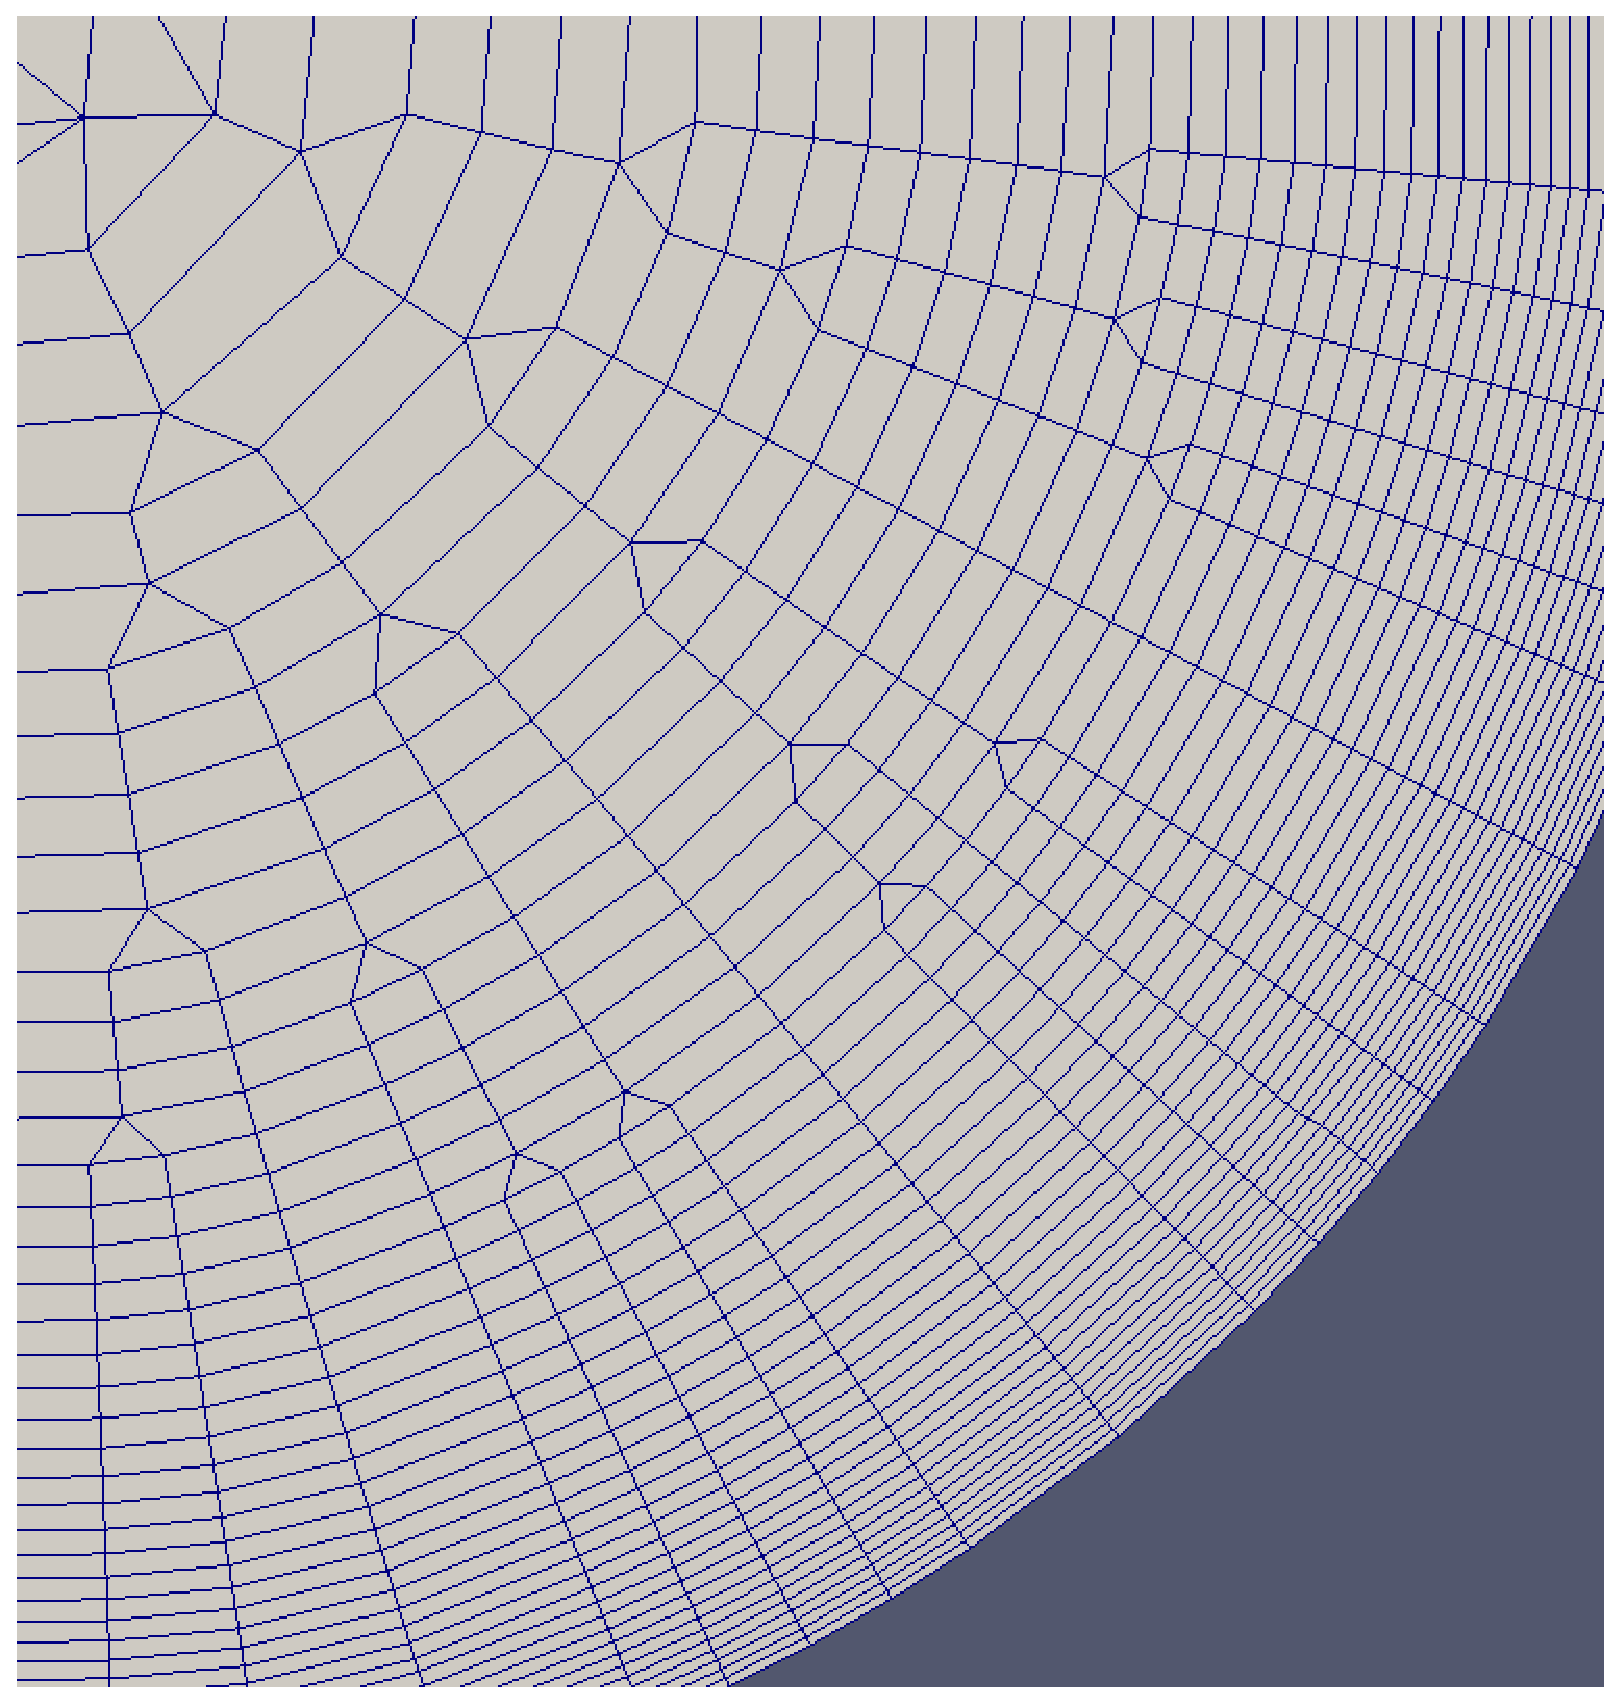
\includegraphics[width =0.9\linewidth]{img/m2/combine-tris-to-quads/combineTrisToQuads2.eps}
		\caption{}
		\label{fig-triQuad2}
	\end{subfigure}
	\caption[Combining triangular cells to quadrilateral cells in EDAMSurf.]{Combining triangular cells to quadrilateral cells based on the quality of the quadrilateral cells generated. For any given quadrilateral element, the inverse of the maximum deviation of its interior angles from 90$^\circ$ is adopted as the measure of quality.}
	\label{fig-triQuad}
\end{figure}

\section{Mesh Smoothing}

Mesh smoothing is the process of improving the quality of the mesh by moving vertices. However, the context in which quality is referred to changes with the application of the mesh. The diffusion of mesh elements might be a desirable effect of mesh smoothing in one application and might not be a desirable effect in another application. One class of mesh smoothing techniques filters out noise in the vertex spacing at high frequencies. Laplacian smoothing is the simplest example of such a smoothing technique. In a very simplistic Laplacian Smoothing technique, vertices in the mesh are moved towards the average position of its neighbors. Another implementation considers moving the centroid of an element towards the average location of the centroids of the adjacent elements. In either case, there is a filtration of high-frequency undulations on the surface mesh. This causes loss of sharp features on the surface. Also, such a smoothing methodology results in shrinkage of the volume of the geometry which might not be desirable everywhere. This class of mesh smoothing techniques provides computationally inexpensive methods for mesh smoothing. However, there is no guarantee that the quality of the mesh would improve or the resultant mesh would even be valid.

Another class of mesh smoothing methodology falls under the category of optimization by minimizing a given energy or error function in the mesh \cite{freitag1997tetrahedral, zhou2000angle, chen2004mesh, parthasarathy1991constrained, shephard1991automatic}. Here, an optimal new location of each vertex is found out using some optimization techniques. These methods, unlike Laplacian smoothing methods, provide guaranteed validity and improvement in the mesh. However, the computational cost of these techniques is much higher. The last class of techniques we will talk about is the Combined Laplacian and Optimization Based Mesh Smoothing techniques\cite{freitag1997combining, canann1998approach}. Such techniques try to combine the benefits of both techniques. Some sort of smart Laplacian Smoothing is followed by Optimization-Based Smoothing in such methods.

All the mesh smoothing techniques we discussed until now apply well to isotropic meshes but do not give satisfactory results for boundary layer meshes. Optimization or Laplacian Smoothing techniques tend to diffuse out the anisotropy in boundary layer meshes. Hence, another class of smoothing technique, called physically-based smoothing technique is generally used to smooth boundary layer meshes \cite{numerow2017mixed, liu2016automatic, xu2006angle, lin2014vertex}. For our mesh generation scheme, we choose a physically-based smoothing technique. The mesh vertices (or nodes) on the mesh exert forces on adjacent nodes. Subsequently, the mesh nodes move to balance out these forces and reach a local force balance equilibrium. This method of smoothing is also referred to as spring-based smoothing methodology as each edge (or link) in the mesh acts as a spring which pushes or pulls its endpoints away or towards each other.

\begin{figure}
	\centering
	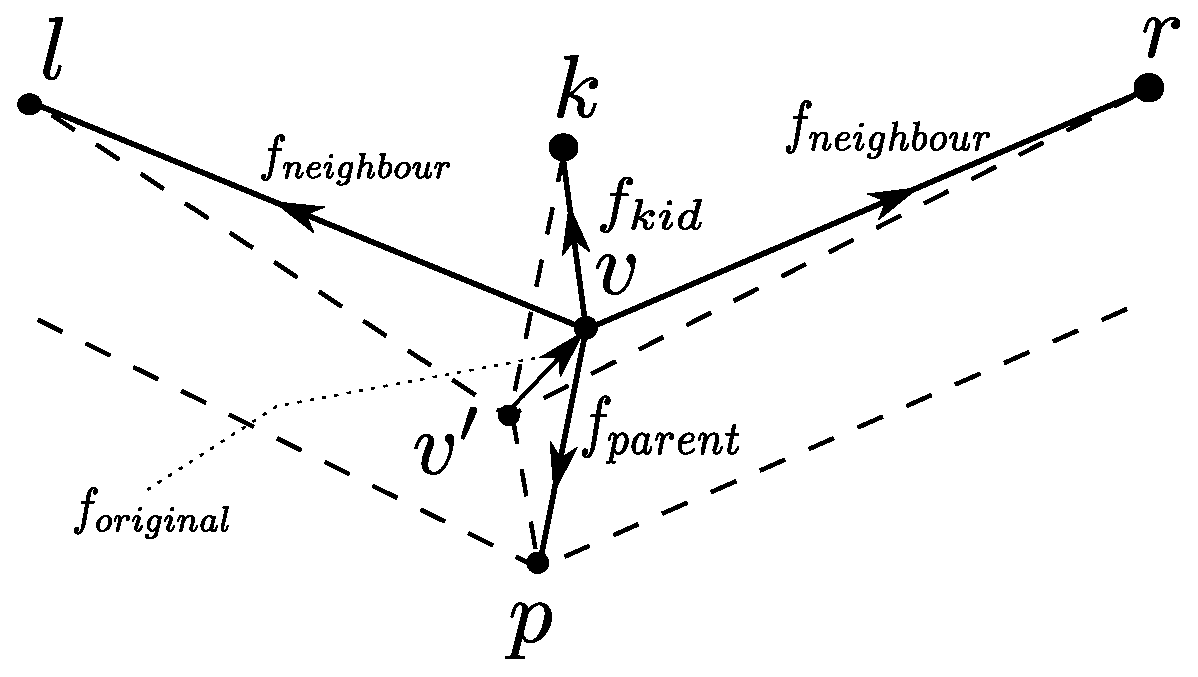
\includegraphics[width=0.7\linewidth]{img/m2/smoothing/smoothing.eps}
	\caption[Smoothing force components on a vertex.]{Smoothing Forces. Force $k_{parent}$ keeps the distance between the parent vertex $p$ and the current vertex $v$ close to ideal. Force $k_{kid}$ is a similar force which keeps the distance between the kid vertex $k$ and $v$ close to ideal. Force $f_{neighbour}$ pushes the vertex $v$ towards the center of the left and right vertices, $l$ and $r$, respectively. After the vertex $v$ has moved under the influence of these three forces to a new location $v'$, a force $f_{original}$ pulls the the vertex, now at $v'$ to its original position $v$.}
	\label{smoothingForces}
\end{figure}

Choosing a spring-based smoothing methodology gives us freedom to select the proportion of forces applied in the extrusion direction and along the advancing layer direction. The proportion can be changed by changing the spring constant of the springs associated with the edges in either direction. Several spring forces are applied to a given mesh node in the smoothing procedure. Each spring constant is denoted by $k_{spring}$. The forces are:


\begin{itemize}
	\item \textbf{Parent force} - force which keeps the distance of the vertex to its parent (from which it was extruded) close to the initial extrusion length, $\mathit{l_{ideal}}$, between the two.
	\begin{equation}
	\mathit{f_{parent}} = \mathit{k_{extrusion}} \cdot \frac{l_{real} - l_{ideal}}{l_{real} + l_{ideal}} \cdot \norm{ \vec{p} - \vec{v}}
	\end{equation}
	\item \textbf{Kid force} - similar to the parent force, this one keeps the distance between the node and its kid close to the initial extrusion length.
	\begin{equation}
	\mathit{f_{kid}} = k_{extrusion} \cdot \frac{l_{real} - l_{ideal}}{l_{real} + l_{ideal}} \cdot \norm{\vec{k} - \vec{v}}
	\end{equation}
	\item \textbf{Neighbour force} - force to maintain uniform spacing of mesh nodes for each layer.
	\begin{equation}
	\mathit{f_{neighbour}} = k_{neighbour} \cdot \frac{(\vec{v} - \vec{l}) + (\vec{v}- \vec{r})}{ 2}
	\end{equation}
	\item \textbf{Original location} - a force is added to restrict the movement of the vertex from the location at which it was placed in the mesh before smoothing. This term also ensures that the deviation of the mesh nodes from the initial surface representation is as little as possible.
	\begin{equation}
	\mathit{f_{original}} = k_{original} \cdot (\vec{v}- \vec{v'})
	\end{equation}
\end{itemize}

These forces are summed up to give the mesh node a resultant force and the node is moved according to the total force. Several iterations (around 5-10) of smoothing are done per layer as the mesh advances towards the surface interior. A limit is set to the vertex movement per smoothing iteration. The distance a vertex moves per iteration of the smoothing algorithm is kept at $5\%$ of the extrusion length at that vertex. This helps in limiting the movement of the vertex when the initial boundary discretization is too coarse. The limitation of choosing a spring-based smoothing technique is that we have to carefully identify the spring constants, $\mathit{k_{spring}}$ for our algorithm. However, once these constants are identified, they seem to work reasonably well for all the cases that we run. The value of $\mathit{k_{extrusion}}$ we use is 0.01, $k_{neighbour}$ is kept at 0.02 and $\mathit{k_{original}}$ at 0.1. Figure \ref{fig-smoothing-cylinder} shows an advancing layer surface mesh with and without smoothing applied to the mesh vertices. It can be seen that smoothing helps improve the vertex spacing along the advancing layer, thereby making the aspect ratio more uniform at a given front.

\begin{figure}
	\centering
	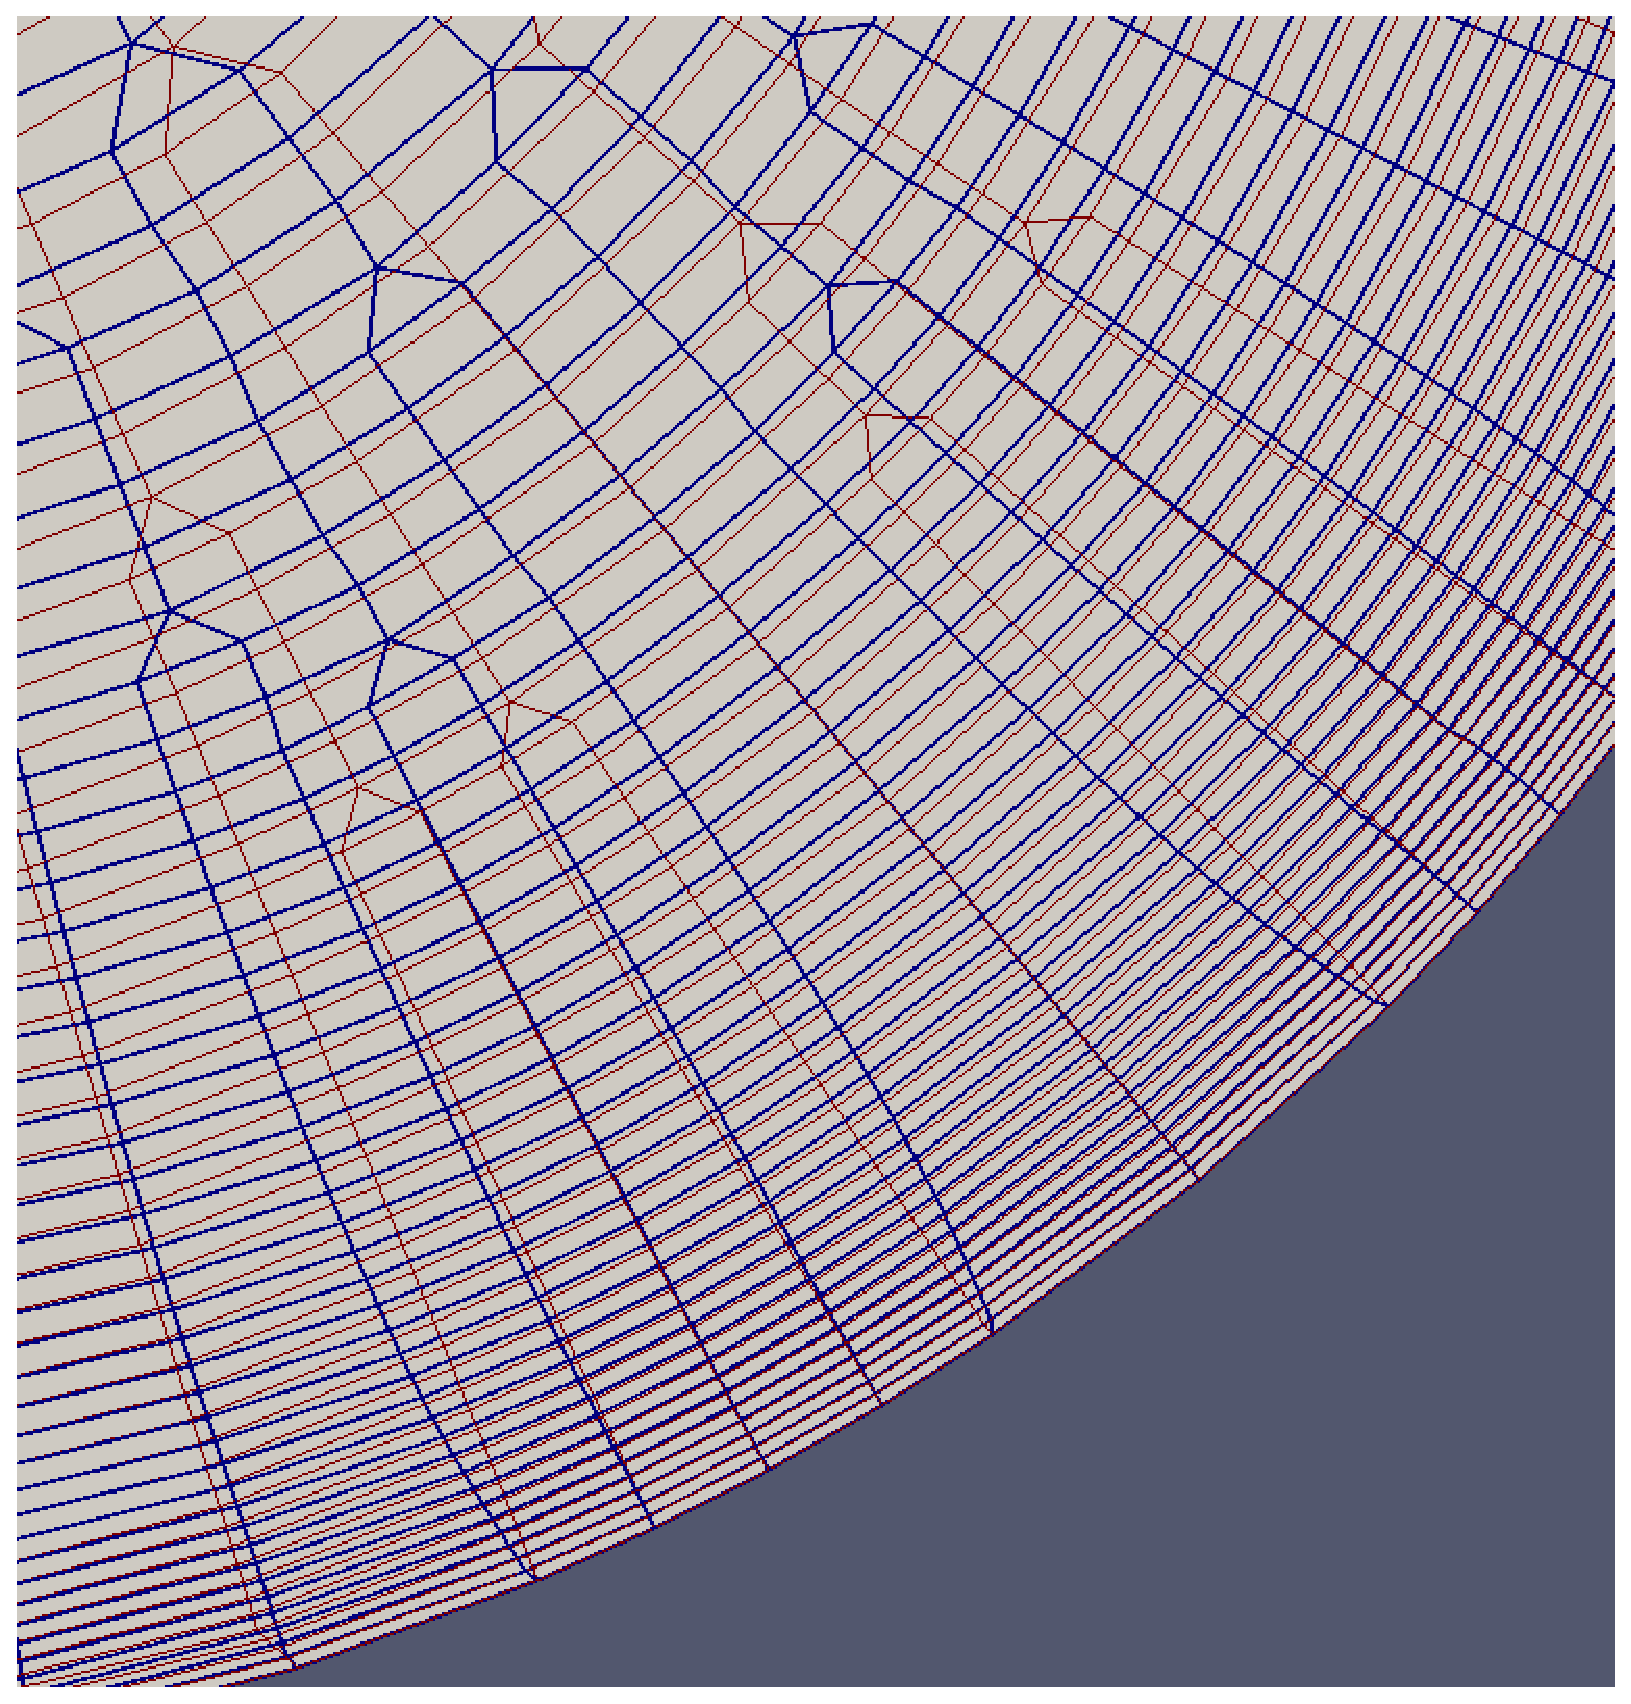
\includegraphics[width=0.4\linewidth]{img/m2/smoothing/smoothing-comparison-cylinder-cap.eps}
	\caption[Comparison of a surface mesh before and after smoothing is applied.]{Zoomed-in view of smoothing applied to an advancing layer surface mesh. Dark blue lines represent the smoothed mesh and flat red lines represent the mesh without smoothing. We can see that the smoothed version of the mesh helps to attain a uniform aspect ratio at each layer.}
	\label{fig-smoothing-cylinder}
\end{figure}

\section{Collision Handling}
\label{collisionHandling}

In our surface mesh generation scheme, we take several measures to avoid or delay advancing front collisions. The extrusion length scaling subroutine, described in Section \ref{extrusionLengthScaling}, scales the extrusion length at a vertex on the front to output better quality quad cells at concave corners. This helps us delay front collisions at such sites in the mesh. Vertex decimation on the front, explained in section \ref{aspectRatioControl}, along with controlling aspect ratio, also helps avoid front collapse when two front vertices come sufficiently close to each other. Mesh smoothing, described in the last section also helps in avoiding front collapses to some extent. Despite undertaking such measures, front collapses at sharp concave corners and head on front collapses at mesh closure zones (where the fronts from two different regions of a sub-surface collide) are inevitable. Hence, subroutines for handling front collisions are important to get a complete surface mesh.

We classify how two advancing fronts may collide into two categories. The first one is the front collision near a sharp corner. Here, the advancing fronts from either side of the sharp corner can collapse onto each other. In the next section, we will discuss how the front collisions are handled in such cases. A second way in which fronts can collide is when two fronts from different regions of a sub-surface march until the point where they come sufficiently close to each other. If the fronts keep marching, front collision is inevitable and there needs to be a subroutine to stop the vertices which are in close proximity to other vertices on the front from marching further. Figure \ref{fig-collisionIllustration} shows an illustration of these two scenarios of advancing front collision.

\begin{figure}
	\centering
	\begin{subfigure}{0.5\textwidth}
		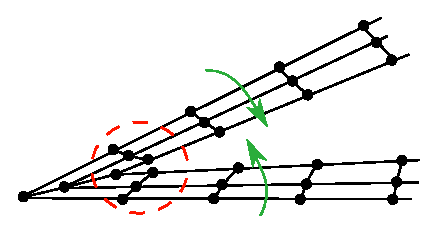
\includegraphics[width=0.9\linewidth]{img/m2/cornerCollision/cornerCollisionIllustration.eps}
		\caption{}
		\label{fig-cornerCollisionIllustration}
	\end{subfigure}%
	\begin{subfigure}{0.5\textwidth}
		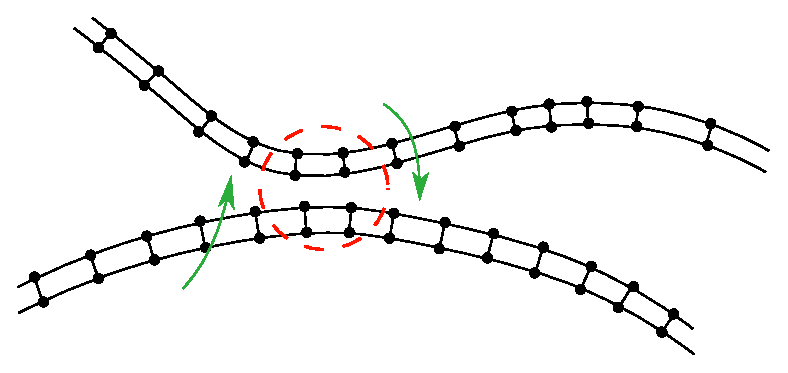
\includegraphics[width =0.9\linewidth]{img/m2/headOnCollision/headOnCollisionIllustration.eps}
		\caption{}
		\label{fig-headOnCollisionIllustration}
	\end{subfigure}
	\caption[Two ways of front collision --- corner collision and head on collision.]{Illustration of the two ways in which advancing front collisions have been categorized. Green arrows show the approximate direction of front advancement. Red dashed circle denotes the region where front collision is about to occur. (a) Collision at concave corners. Sections of the front from the left and the right side of the corner tend to collide onto each other as they advance towards the front interior. Scaling extrusion lengths, explained in section \ref{extrusionLengthScaling}, helps delay or avoid such collisions. (b) At the regions of the surface mesh where meshing is about to complete, advancing fronts would collide onto each other as shown.}
	\label{fig-collisionIllustration}
\end{figure}

\subsection{Collisions at Concave Corners}
\label{collisionConcaveCorner}

For concave corners of the mesh which might collide onto themselves, we preemptively close off the corner before the layers collide. Consider a concave corner as shown in figure \ref{fig-cornerCollision}. Point $A$ is a corner vertex at the mesh front $CAB$. The extrusion length at the front is $h$. The length of the edge $AB$ is $l$. If point $B$ is extruded with the current front definition, the extruded point $D$ would cross the angle bisector of $\angle BAC$, $AX$, and will invalidate the front. This is likely to occur for smaller aspect ratio ($\AR$)  values and small values of included angle $2 \, \theta$. To avoid collisions in the next front, we insert a new point $F$ into the mesh, located at the surface projection of the mid-point of $B$ and $C$. $F$ takes the place of $A$ as a front vertex and this procedure is repeated until no point which is extruded from the front crosses the angle bisector of its neighbors. The value of angle $\theta$ where this occurs can be written as $\theta = \tan^{-1}(1/\AR)$, where $\AR$ is the aspect ratio at the corner vertex. Hence, we identify a corner as any vertex on the front which has half interior angle $\theta$ less than a threshold time this limit.
\begin{equation}
\mathit{\theta_{corner} < threshold * \tan^{-1}(1/\AR)}
\label{eqn-corner-threshold}
\end{equation}

The threshold is taken as 1.5 for our mesh generation method to resolve all corner collision instances.

\begin{figure}
	\centering
	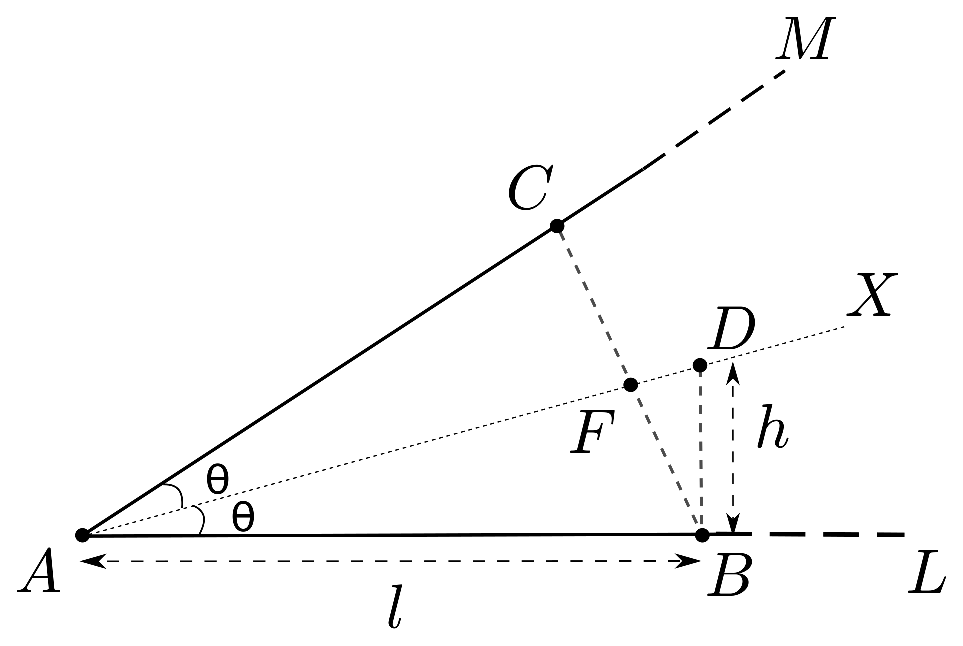
\includegraphics[scale=0.4]{img/m2/cornerCollision/cornerCollision.eps}
	\caption[Handling collisions at concave corners]{Handling collision at concave corners to avoid layer overlap. Corner point $A$ is replaced by point $F$ so as to form the new front $CFB$. $F$ is the surface-projected mid-point of points $B$ and $C$. This corner collision handling is done until all the half-interior angles, $\theta$ are within the limit described by equation \ref{eqn-corner-threshold}.}
	\label{fig-cornerCollision}
\end{figure}

The concave corner detection subroutine works well to close off the corners. However, the vertex placement at such concave corners is not ideal every time. It tends to produce skinny triangular elements if there are multiple corners adjacent to each other because of bad boundary discretization. Hence, this is a limitation of the current formulation. Figure \ref{fig-cornerLimitation} shows such a case. A zoomed-in view of the trailing edge of an airfoil is shown. Two sharp corners at the boundary of the surface are successfully closed by the mesh and the front continues to advance towards the interior of the surface. However, the quality of the triangular elements generated is not ideal. Better vertex placement and a different smoothing subroutine for such vertices could produce better quality mesh elements for such cases.

\begin{figure}
	\centering
	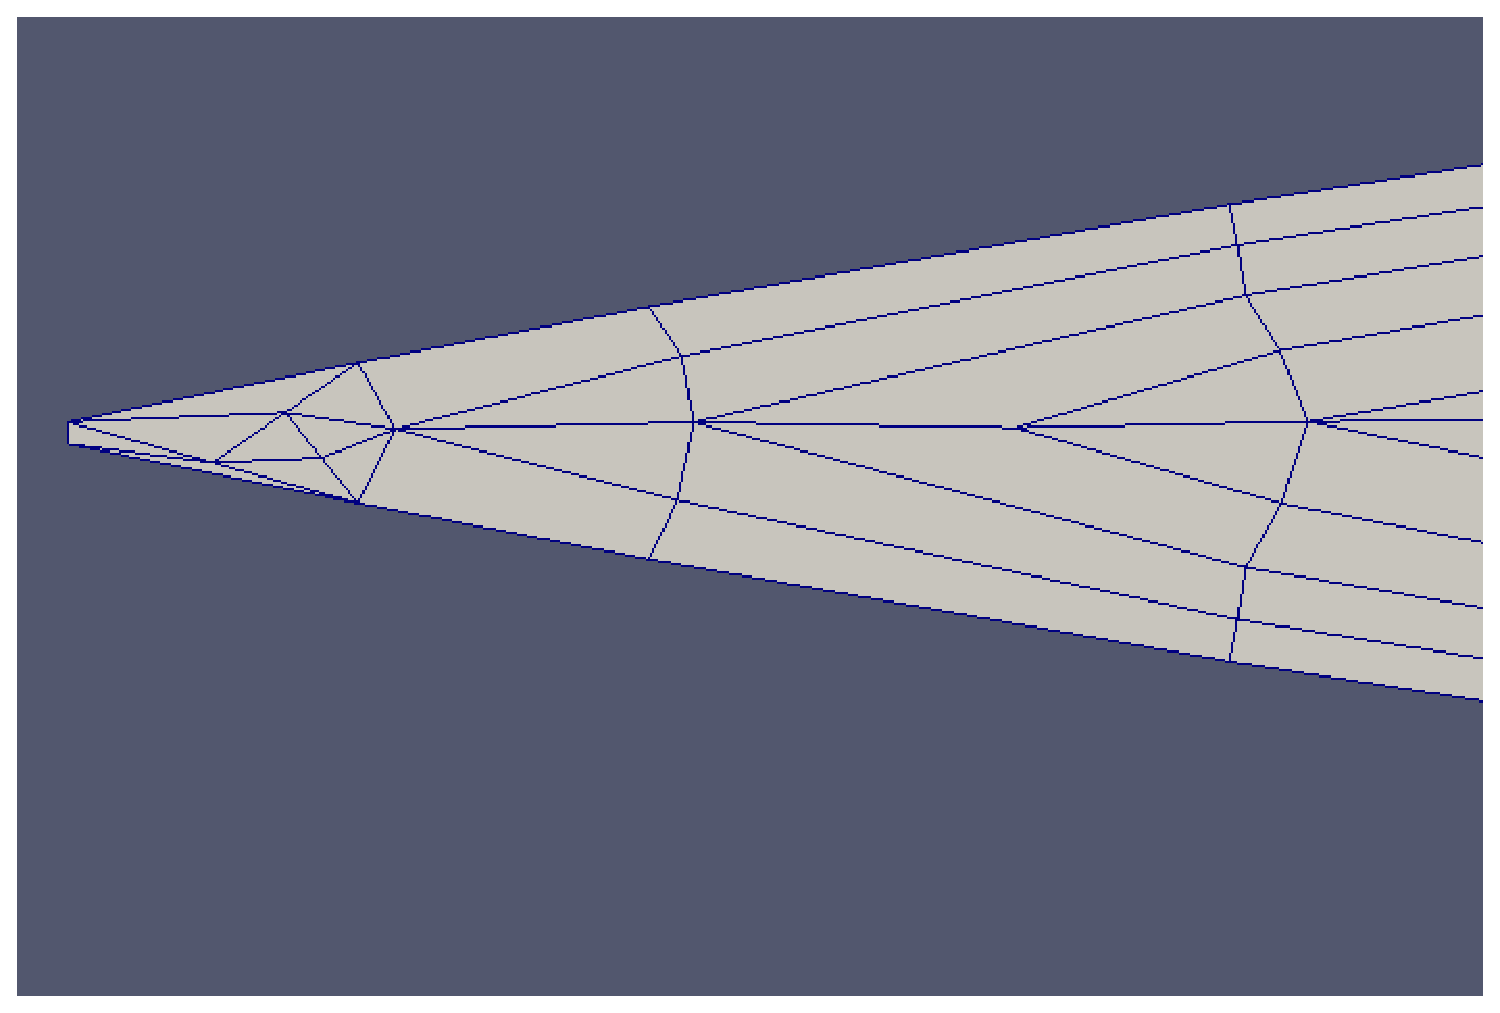
\includegraphics[width=0.4\linewidth]{img/m2/cornerCollision/cornerLimitation.eps}
	\caption[Limitation of the concave corner collision detection and front redefinition subroutine.]{Limitation of the concave corner collision detection and front redefinition subroutine. Zoomed-in view of the trailing edge of an airfoil is shown. The subroutine successfully closes off the two concave corners present a the tip of the trailing edge, but produces a couple of skinny triangles in the mesh with non-ideal vertex placement.}
	\label{fig-cornerLimitation}
\end{figure}

\subsection{Head-On Collisions}

\begin{figure}[!hbt]
	\centering
	\begin{subfigure}{.5\textwidth}
		\centering
		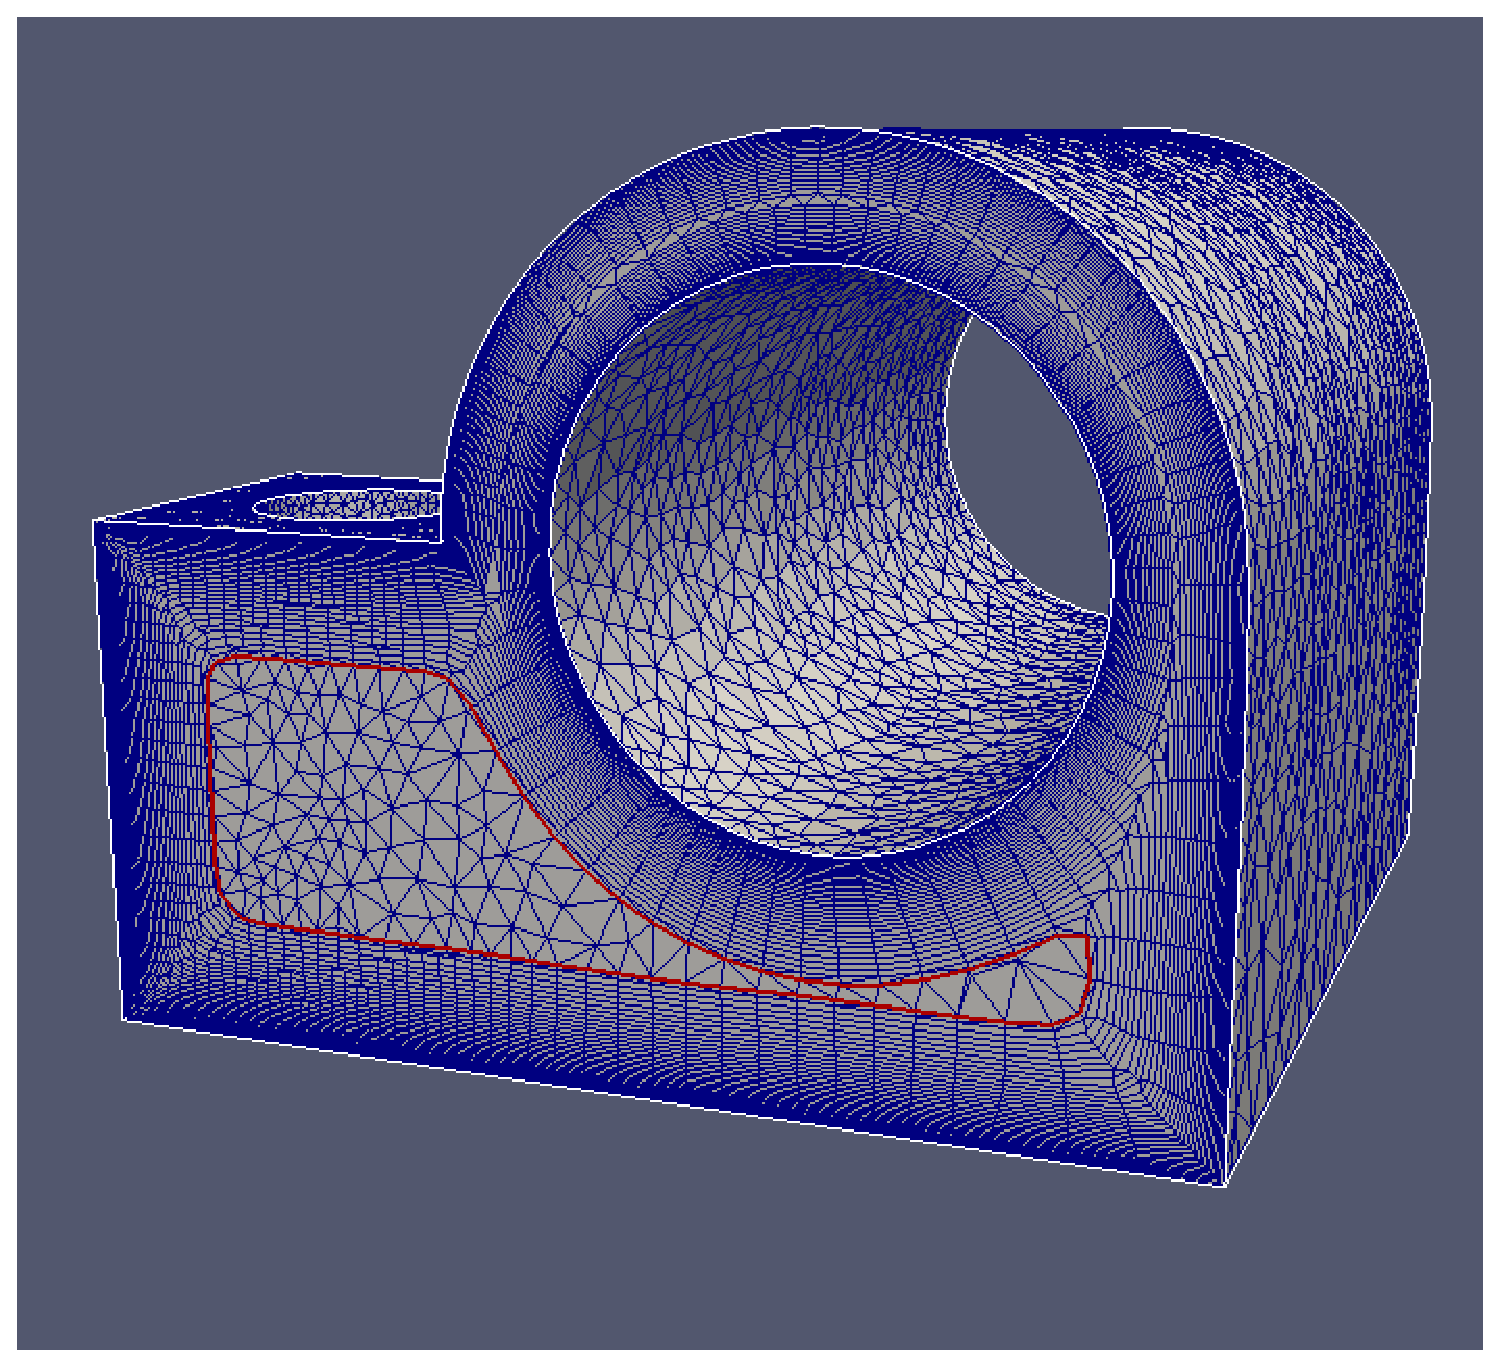
\includegraphics[width=.9\linewidth]{img/m2/meshCases/joint-x0.004-g1.04-a5/collapse1.eps}
		\caption{}
		\label{fig-collision1}
	\end{subfigure}%
	\begin{subfigure}{.5\textwidth}
		\centering
		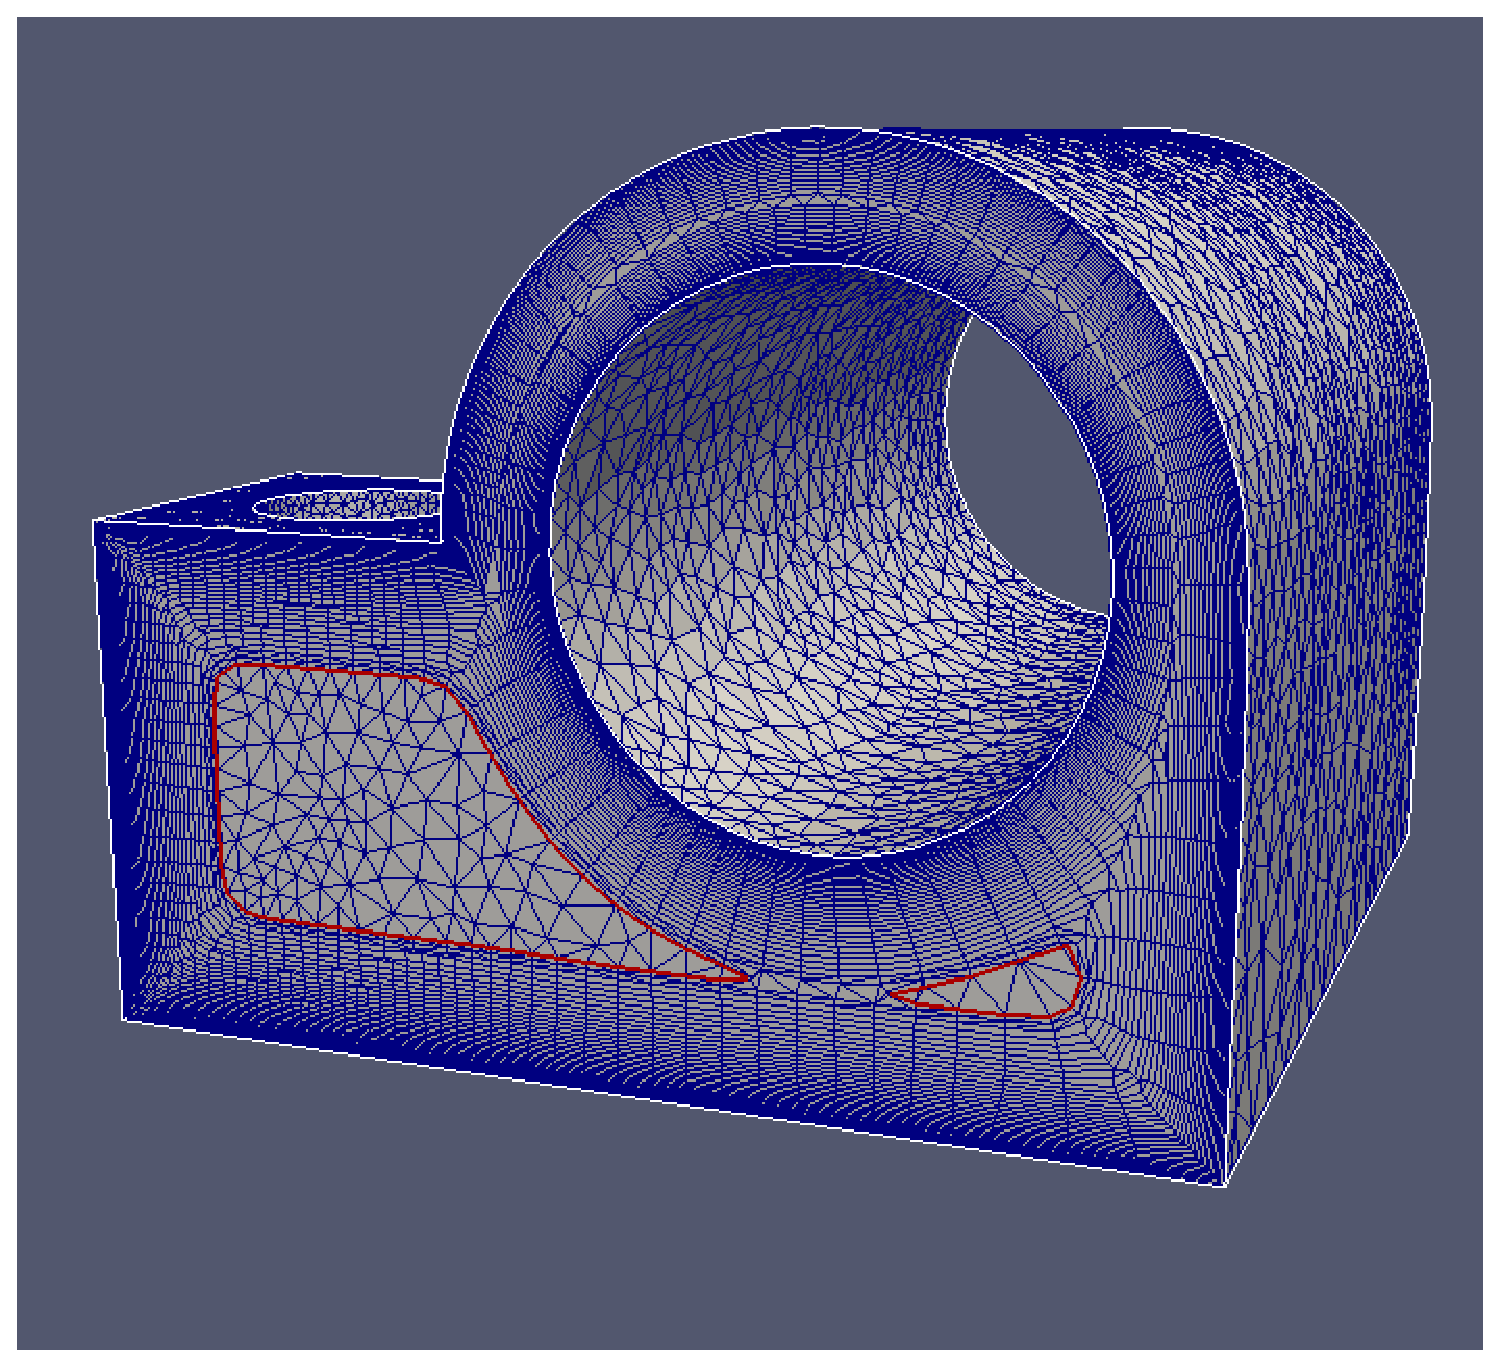
\includegraphics[width=.9\linewidth]{img/m2/meshCases/joint-x0.004-g1.04-a5/collapse2.eps}
		\caption{}
		\label{fig-collision2}
	\end{subfigure}
	\caption[Handling head-on front collisions.]{Handling front collisions. (a) shows an advancing front which is about to collide onto itself. Using the vertex connectivity at the advancing layer and the proximity of the advancing layer vertices from each other, some of the front vertices are removed from the front and the front is redefined. The redefined front extruded to the next layer is shown in (b). From this iteration of the front, it would proceed with only the vertices on the front shown in red.}
	\label{fig-collision}
\end{figure}

Apart from handling collisions at the corners of the mesh, we also need to take care of the front collisions which happen elsewhere. Consider Figure \ref{fig-collision1} where the advancing layer surface mesh generation algorithm is meshing one of the surfaces of the geometry shown earlier in Figure \ref{fig-surfSegment}. The advancing front is shown in red in the figure. After advancing several layers from the boundary, it reaches a point where it is about to collapse onto itself. Hence, some sort of front redefinition is necessary before moving on to the next layer. To achieve this, we first iterate through all the points on the front to identify the encroached points. These points are the ones whose distance from any edge in the front, except its adjacent edges, is less than a threshold (taken as $2.4$) times the extrusion length at that point. As our surface mesh is closed, we can utilize the vertex connectivity to find possible vertex-front edge encroachment. Hence, for a given point on the advancing front, only the edges on the front that share a triangle with that point are checked for encroachment. This saves a lot of computational cost while identifying encroached vertices. We assume that the input boundary discretization and surface triangulation are fine enough to resolve the complex features of the geometry so that we don't have to iterate through all the edges on the front to find whether a given point is encroached or not.

After these encroached points and their corresponding edges are identified, we reconnect the non-encroached points in order to form the new front. The encroached points are moved out of the advancing front and the front is hence redefined. In Figure \ref{fig-collision2}, we show the redefined front extruded to the next layer. In this case, the front is divided into two loops, each of which continues to march independently towards the interior of the surface. After dealing with the concave corner collision cases, this approach helps us tackle front collisions at other regions of the front and completes the front redefinition process wherever the advancing front might collide onto itself.

\section{Overall Mesh Generation Algorithm}
In the previous section, we have detailed the steps in the advancing layer mesh generation routine. Here, we summarize the algorithm in the form of pseudo-code in Algorithm \ref{algo}.

\begin{algorithm}[hbt!]
	\caption{Overall Mesh Generation algorithm}\label{alg:euclid}
	\begin{algorithmic}[1]
		\Procedure{SurfMesh::CreateMesh}{triangulation $T,$ extrusion length, growth ratio}
		\State Create surface geometry $S \gets T$
		\State Initialize advancing layer $F$ from surface boundary
		\While{ $F\neq\emptyset$}\Comment{Advance until Front $F$ is empty}
		\State \textsc{AdvanceLayer($F$)}
		\State Validate the new Layer
		\EndWhile \label{advancing-layer-routine}
		\State Export \textsc{SurfMesh}
		\EndProcedure
		\Procedure{SurfMesh::AdvanceLayer}{$F$}
		\State Delete encroaching interior vertices
		\State Redefine front $F$ until no vertex encroachment \Comment{Take care of collisions}
		\State Extrude all points of $F$ and Insert Into Mesh
		\State Recover front $F'$ \Comment{Through forced edge creation between kid vertices}
		\State Improve mesh quality by edge swapping \Comment{In the immediate interior of mesh}
		\State Collapse short edges in the front
		\State Combine triangular elements to quads
		\State Smooth vertices
		\State Update extrusion length for vertices
		\EndProcedure
	\end{algorithmic}
	\label{algo}
\end{algorithm}

\section{Assumptions}

We make a few assumptions on the input triangulation for our mesh generation algorithm to successfully create a valid mesh. The first one is that the triangulation of the surface is fine enough to resolve the geometric complexities in the object. If the input triangulation is too coarse, the encroaching interior vertex deletion subroutine will create mesh elements that deviate significantly from the surface. This might lead to failure to generate a valid mesh front in the next step. Hence, for highly curved regions of the surface, the maximum deviation between any triangle in the initial input triangulation of the body and the underlying surface that it represents should be limited to 30 degrees. However, this issue can be tackled by refining the triangulation using any isotropic refinement algorithm as long as it retains the features of the input object. Coarse triangulations are acceptable for objects without any geometric complexities.

Another assumption we have made for the input triangulation is that it would have well-defined boundaries where the advancing layers can march out from. Sharp corners in the input geometry are automatically identified as boundaries of the mesh but the boundary discretization of blunt corners needs to be supplied as an input to the advancing layer surface mesh generator.